
%% url is loaded by the document class, so its options have to be registered
%% before \documentclass. Loading it again with [hyphens] causes an option clash.
\PassOptionsToPackage{hyphens}{url}

\documentclass[blue]{ludusofficial}  % Theme: blue, red, green, purple, orange, cyan
                                               % Article type: fullpaper, letter, poster, survey, shortpaper, artpaper

%% Document metadata
% BibLaTeX Vancouver-like numeric refs, but truncate authors to 1 + et al.
\usepackage{amsmath}
\usepackage{graphicx}
%% dblfloatfix is deliberately not loaded. It pulls in fixltx2e, which is
%% obsolete on TeX Live 2015 and later and aborts the build. It was only needed
%% to place double-column floats at the bottom of a page, and this manuscript
%% has no figures.
\usepackage{placeins}
\usepackage{lineno}
%% Without these, LaTeX defers most floats to the end of the document in a
%% two-column layout. They let more floats sit at the top of a page and allow a
%% page to be mostly float.
\setcounter{topnumber}{4}
\setcounter{dbltopnumber}{4}
\setcounter{bottomnumber}{2}
\setcounter{totalnumber}{6}
\renewcommand{\topfraction}{0.95}
\renewcommand{\dbltopfraction}{0.95}
\renewcommand{\bottomfraction}{0.5}
\renewcommand{\textfraction}{0.05}
\renewcommand{\floatpagefraction}{0.8}
\renewcommand{\dblfloatpagefraction}{0.8}
\linenumbers

%% Article information
\title{Longitudinal Boundary Sharpness Coefficient Slopes and Clinical Covariates for Prediction of Alzheimer's Disease Conversion in Mild Cognitive Impairment: A Survival Analysis Using the ADNI Cohort}

\shorttitle{Follow-up Definition and BSC Slopes in MCI}  % Short title for page headers
\shortauthor{Cherukuri}  % Short author names for page headers

\author{%
    \textbf{Ishaan Cherukuri}\textsuperscript{1}\textsuperscript{*}\\[0.2cm]
    \small\textsuperscript{1}Douglas Research Centre, Montreal, QC, Canada\\
    \small Corresponding: ishaan.cherukuri@gmail.com\\[0.4cm]
    \small\textsuperscript{*}Data used in preparation of this article were obtained from the Alzheimer's Disease Neuroimaging Initiative (ADNI) database (adni.loni.usc.edu). As such, the investigators within the ADNI contributed to the design and implementation of ADNI and/or provided data but did not participate in the analysis or writing of this report. A complete listing of ADNI investigators can be found at: \href{http://adni.loni.usc.edu/wp-content/uploads/how_to_apply/ADNI_Acknowledgement_List.pdf}{adni.loni.usc.edu/how\_to\_apply/ADNI\_Acknowledgement\_List.pdf}
}

\begin{document}

%% Abstract and keywords must be defined BEFORE \maketitle
\begin{abstract}
The Boundary Sharpness Coefficient (BSC)\cite{olafson2021bsc} measures how well-defined the gray-white matter boundary looks on structural MRI, and annualized change in BSC has been proposed as a prognostic marker for progression from mild cognitive impairment (MCI) to Alzheimer's disease (AD). Structural MRI is attractive for this purpose because it is already part of standard workups and costs a fraction of PET imaging. This study evaluates that proposal in the ADNI cohort under a follow-up definition in which features come only from scans acquired while the subject was still MCI and the survival clock starts at the last such scan, giving 2,252 scans from 417 subjects (133 converters, 284 stable). Because longitudinal imaging studies vary in whether they impose this restriction, the same models were also fitted under the looser definition that permits scans acquired after the dementia diagnosis, so that the two designs could be compared directly. Clinical covariates, cortical thickness and hippocampal volume comparators, longitudinal ComBat harmonization and a 62-parcel regional analysis were added. Clinical covariates alone reached a cross-validated C-index of 0.795, global BSC slopes 0.584 and regional BSC slopes 0.649. Fold-matched comparisons showed no incremental value for BSC over covariates and standard longitudinal MRI (change in C-index 0.002, 95\% CI $-0.021$ to $0.022$). Restricted to the same 417 subjects, the corrected definition cost covariates 0.010 to 0.034 in C-index but cost every imaging family two to four times more. The null survived two sensitivity analyses: treating the 28 deaths that preceded a dementia diagnosis as a competing event rather than as censoring, and restricting to the 188 amyloid-positive subjects with 81 events. Two lines of evidence bear on why. BSC showed no association with age ($r=-0.007$, $p=0.74$) and none with any amyloid or tau biomarker after correction, while tracking signal-to-noise ratio more strongly within a single brain over time ($+0.30$ per SD, 95\% CI $+0.17$ to $+0.43$) than across scans ($r=0.191$); and a model given nothing but scanner identity reached a C-index of 0.609, above global BSC slopes. The prognostic value previously attributed to BSC slopes is therefore better attributed to the follow-up definition and to acquisition than to the biomarker.
\end{abstract}


\keywords{Alzheimer's disease; mild cognitive impairment; boundary sharpness coefficient; longitudinal MRI; survival analysis; guarantee-time bias; competing risks; construct validity; scanner harmonization; ComBat; amyloid; MCI-to-AD conversion; ADNI; null result; reproducibility}

%% Maketitle creates full-width header with abstract and keywords, then starts two-column layout
\maketitle

%% From here, content is in two columns
\section{Introduction}

Dementia affected an estimated 57 million people worldwide in 2019 and is forecast to reach 153 million by 2050~\cite{gbd2022dementia}, with Alzheimer's disease its leading cause. Mild cognitive impairment (MCI) sits in a more uncertain space, since it is neither normal aging nor dementia, and it does not lead everyone down the same path. A meta-analysis of 41 inception cohorts put the annual conversion rate to dementia near 5 to 10\%~\cite{mitchell2009rate}, but that average hides wide variation. Some individuals remain stable for years, some improve, and others decline quickly.

The clinical need for early risk stratification has grown with the arrival of anti-amyloid therapies such as lecanemab~\cite{vanDyck2022lecanemab} and donanemab~\cite{sims2023donanemab}, which target earlier disease stages. Amyloid PET measures pathology directly but costs \$5,000--\$7,000 per scan and is not widely accessible. Cerebrospinal fluid testing is invasive. Blood-based biomarkers are advancing quickly, though interpretation is still not entirely straightforward. Structural MRI is already part of standard workups for cognitive complaints and costs roughly \$800--\$1,500. The difficulty is that conventional MRI markers measured at a single time point have often disappointed for prediction~\cite{ansart2021predicting}.

MCI-to-AD prediction has a substantial literature, and two systematic reviews map it. Ansart et al.~\cite{ansart2021predicting} reviewed 234 experiments drawn from 111 articles and asked which data types actually improved prediction. Cognitive testing, FDG-PET and electrophysiological measures each improved performance significantly, whereas adding T1-weighted MRI did not. Grueso and Viejo-Sobera~\cite{grueso2021machine} screened 452 studies and analyzed 116, and noted that few validate externally. The Ansart result is a specific quantitative prediction: a T1-derived marker should not add value once cognition is in the model. The present study provides one such test.

Time-to-event modeling of AD progression is likewise well established. Da et al.~\cite{da2014integration} combined the SPARE-AD atrophy index with cognitive scores, APOE genotype and CSF biomarkers in a Cox framework, and found that cognitive measures carried much of the predictive weight. Li et al.~\cite{li2017prediction} jointly modeled longitudinal biomarkers with time to conversion in ADNI. Zhang et al.~\cite{zhang2024interval} modeled conversion time directly with interval-censored methods, which acknowledges that conversion is observed only at discrete clinic visits rather than on the day it occurs. Across these studies a consistent pattern appears: once cognitive and demographic information is in the model, additional imaging measures add less than their standalone performance suggests.

That pattern sets the standard a new imaging marker has to meet. Reporting that a marker discriminates converters from non-converters is not sufficient, because the relevant question is whether it adds anything to what is already measured in clinic. The present study was designed to answer that question for BSC, and to measure how much the answer depends on when features are permitted to be measured relative to the outcome.

The Boundary Sharpness Coefficient measures how sharply gray matter and white matter are separated on structural MRI. In a healthy brain the transition between cortical gray matter and underlying white matter is fairly crisp on a T1-weighted scan. Gray matter appears darker and white matter brighter because of its myelin content. When disease-related processes disrupt that organization, the interface can become less distinct.

BSC differs from familiar measures such as regional volume or cortical thickness. Those metrics quantify how much tissue remains. BSC instead captures a property of the boundary itself. It is not a microscope-like readout of microstructure, and claiming otherwise would overstate what a 1 mm voxel can resolve. Several processes in AD could plausibly blur the interface, including synaptic loss, tau pathology, myelin degeneration in superficial white matter, and neuroinflammation. None maps one-to-one onto BSC.


BSC is not the first quantitative index of the gray-white junction, and two earlier traditions bear on this work.

Gray-white matter contrast, introduced by Salat et al.~\cite{salat2009age}, samples T1 intensity at fixed distances above and below the gray-white surface and computes a ratio between the two tissue classes. It has been used extensively as a marker of cortical aging, and Salat et al. reported that it declines measurably with age in healthy adults. Gray-white matter blurring was developed independently in the epilepsy literature~\cite{huppertz2005enhanced,blackmon2015cortical} as a lesion-detection tool for focal cortical dysplasia, quantifying focal blur at the junction by comparison against a normative database.

BSC differs from both in a specific way. Gray-white contrast is a ratio of intensities and therefore a measure of the contrast level between tissue classes. BSC is a spatial derivative and therefore a measure of how abruptly the transition occurs. Two brains can share a contrast ratio while differing in how smeared the transition is. The epilepsy blurring measures are engineered for cross-sectional detection of developmental lesions with dramatic local blur, whereas BSC, following Olafson et al.~\cite{olafson2021bsc}, is intended as a continuous measure suited to diffuse progressive change. The concepts overlap; the methodological requirements do not.

A cross-sectional scan mixes influences accumulated across a lifetime. Two people can show the same hippocampal volume for very different reasons: one may have had a smaller hippocampus for years, the other may be mid-neurodegeneration. A single snapshot cannot separate those cases. Cognitive reserve complicates matters further, since some individuals tolerate substantial pathology before symptoms appear.

Rates of change are appealing for exactly this reason. A declining trajectory can reveal ongoing pathology that baseline values obscure. The hypothesis under test is that annualized BSC slopes capture progression dynamics invisible in a baseline scan.

Testing that hypothesis requires care about when measurements are taken relative to the outcome. If features are drawn from scans acquired after a subject has already been diagnosed, the model is describing established disease rather than forecasting it, and any apparent predictive skill is partly an artifact of the design. This concern applies to any longitudinal imaging marker, not to BSC specifically, and quantifying it is one of the aims below.

The present study rebuilds the ADNI cohort so that every feature comes from a scan acquired while the subject was still MCI, with follow-up starting at the last such scan, and then asks four questions of it. How much does the follow-up definition alone change apparent performance, holding subjects, features and models fixed? Do BSC slopes add prognostic information beyond clinical covariates and established longitudinal MRI measures? Does extending BSC from global summaries to regional measures across a cortical parcellation change that answer? And what does BSC covary with, given that sensitivity to scanner and image quality would limit any longitudinal use of it?

The last question is the one that decides how the first three should be read. A marker can fail to add prognostic value for uninteresting reasons, such as a cohort too small to detect a small effect. It is a different matter if the marker turns out to be measuring the scanner. Two analyses below address that directly: whether BSC moves with image quality inside a single brain over time, and whether acquisition structure by itself predicts conversion.

\section{Materials and Methods}

\subsection{Study population}

All data were obtained from the Alzheimer's Disease Neuroimaging Initiative (ADNI) database (\texttt{adni.loni.usc.edu})~\cite{weiner2010adni,petersen2010adni}. ADNI began in 2003 as a public-private effort led by Michael W. Weiner, MD, to determine whether serial MRI, PET, fluid biomarkers and cognitive testing could track the progression of MCI and early AD. Its standardized protocols and repeated follow-up make it well suited to longitudinal work, though like many research cohorts it is not a mirror of routine clinical populations.

A subject entered the analysis if the baseline scan carried an MCI diagnosis, at least four T1-weighted scans were available before conversion or censoring, scans were chronologically ordered with valid acquisition dates, and clinical metadata were complete. Any scan whose own diagnosis code was AD was excluded from feature computation, as was any scan acquired on or after the date of first dementia diagnosis.

Of 1,617 subjects with processed scans, 421 were excluded because the baseline scan was not MCI, 691 because fewer than four scans remained inside the pre-conversion window, and 88 because no positive follow-up time remained after the last usable scan. The final cohort contained 417 subjects, 133 converters and 284 stable, contributing 2,252 scans. Table~\ref{tab:demographics} summarizes the cohort, and Figure~\ref{fig:splot} shows the age distribution and the observation window of every subject. At scan level, 513 scans were dropped for falling at or after conversion and 152 for carrying an AD diagnosis code. All exclusions were logged. Amyloid status, read from PET where it existed and from CSF A$\beta$42 otherwise, could be established before the landmark for 355 subjects (85\%), of whom 188 (53\%) were positive.

That coverage is not the same in the two outcome groups, and the difference runs the wrong way for convenience. Status was available for 101 of 133 converters (76\%) against 254 of 284 stable subjects (89\%, $p<0.001$). The 62 subjects without a measurement have a median landmark year of 2009, against 2014 for the amyloid-positive and 2015 for the amyloid-negative, and 16\% of them were scanned at 3T against 68\% and 86\%. They are, in other words, largely ADNI1 participants enrolled before amyloid PET was part of the protocol, and ADNI1 was also the phase with the highest conversion rate. Their status is missing for a reason connected to the outcome, so the amyloid-restricted analysis below is a sensitivity analysis and not a replacement for the main one.

The cost of this requirement falls almost entirely on converters. Among subjects with an MCI baseline, 665 had four or more scans in total, of whom 293 converted. Requiring four scans before conversion retained only 133 of those converters. A converter who is scanned four times but converts after the second scan cannot contribute, whereas a stable subject scanned four times always can. Any analysis of this kind trades converter count for temporal validity, and the trade is steep.


\begin{table*}[t!]
\centering
\caption{Demographic and clinical characteristics of the corrected cohort}
\label{tab:demographics}
\begin{tabular}{lcccc}
\hline
\textbf{Characteristic} & \textbf{All} & \textbf{Converters} & \textbf{Stable} & \textbf{$p$} \\
 & (N=417) & (N=133) & (N=284) & \\
\hline
Age at landmark (years) & 76.9$\pm$7.6 & 77.7$\pm$7.2 & 76.6$\pm$7.8 & 0.18 \\
Female, n (\%) & 164 (39.3) & 49 (36.8) & 115 (40.5) & 0.52 \\
Education (years) & 16.2$\pm$2.7 & 16.2$\pm$2.7 & 16.2$\pm$2.7 & 0.97 \\
APOE4 carrier, n (\%) & 179 (42.9) & 78 (58.6) & 101 (35.6) & $<$0.001 \\
Amyloid status available, n (\%) & 355 (85.1) & 101 (75.9) & 254 (89.4) & $<$0.001 \\
Amyloid positive, n (\% of measured) & 188 (52.9) & 81 (80.2) & 107 (42.1) & $<$0.001 \\
MMSE & 27.3$\pm$2.6 & 26.2$\pm$2.4 & 27.9$\pm$2.5 & $<$0.001 \\
ADAS-Cog13 & 16.3$\pm$8.2 & 20.9$\pm$7.1 & 14.1$\pm$7.8 & $<$0.001 \\
CDR sum of boxes & 1.72$\pm$1.41 & 2.56$\pm$1.29 & 1.30$\pm$1.28 & $<$0.001 \\
3T at landmark, n (\%) & 281 (67.4) & 67 (50.4) & 214 (75.4) & $<$0.001 \\
Switched field strength, n (\%) & 50 (12.0) & 19 (14.3) & 31 (10.9) & 0.34 \\
Scans in window & 5.40$\pm$1.79 & 4.93$\pm$1.45 & 5.62$\pm$1.90 & $<$0.001 \\
Window span (years) & 4.18$\pm$3.02 & 3.19$\pm$2.19 & 4.65$\pm$3.24 & $<$0.001 \\
Follow-up after last scan (years) & 1.69$\pm$1.86 & 1.91$\pm$1.48 & 1.58$\pm$2.00 & $<$0.001 \\
\hline
\end{tabular}
\end{table*}

\begin{figure*}[t!]
\centering
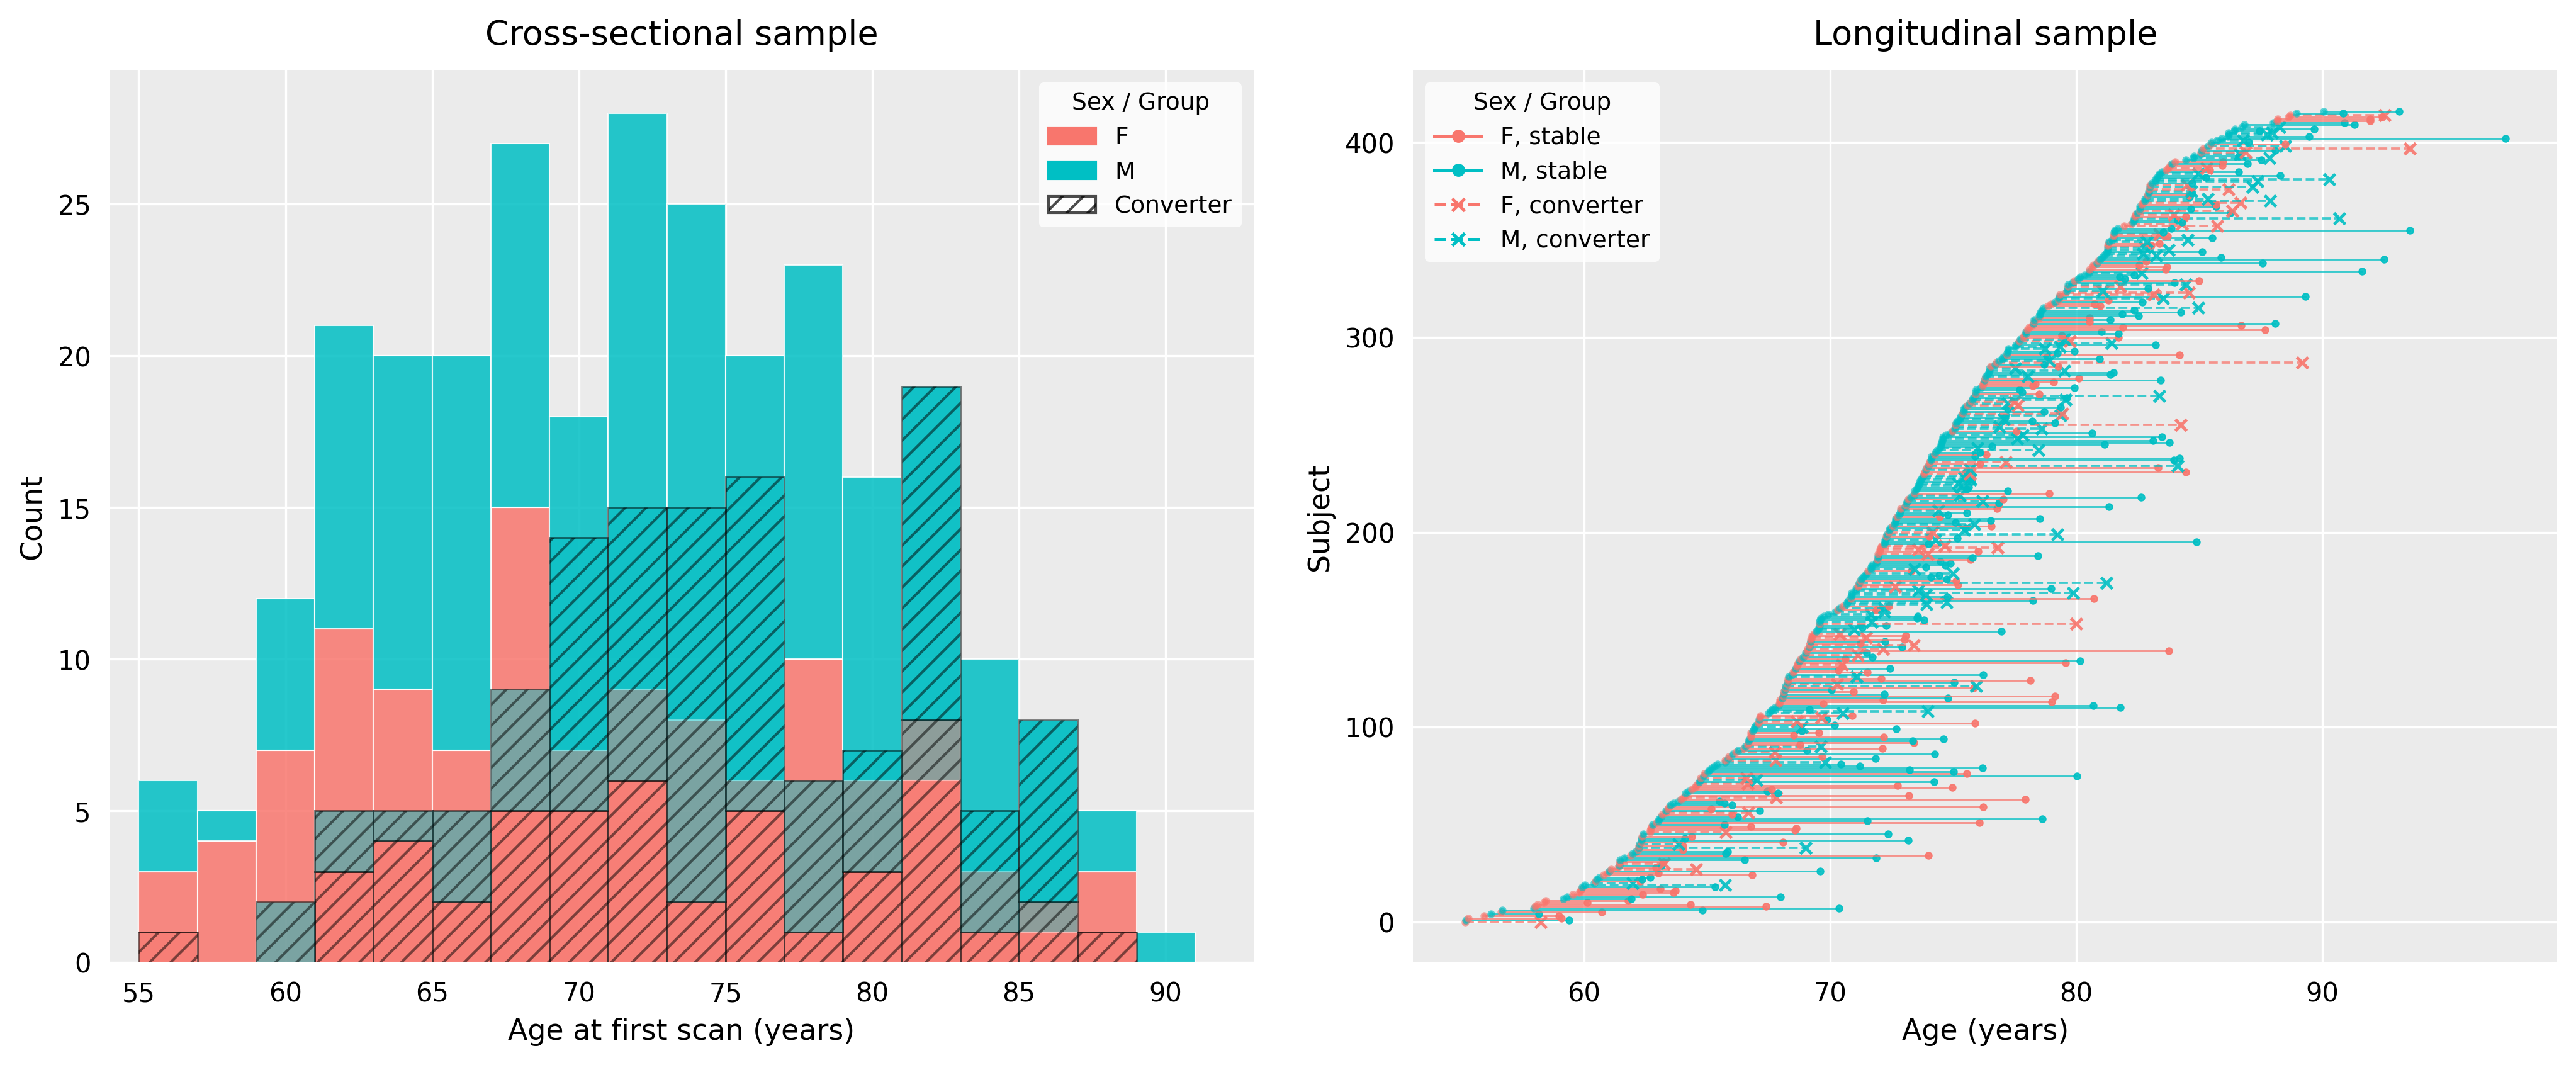
\includegraphics[width=\textwidth]{fig1.png}
\caption{Cohort demographic and longitudinal sampling structure. Left: age
distribution at the first scan, stacked by sex (salmon female, teal male), with
converters overlaid as hatched bars. Right: observation window for each of the
417 subjects, sorted by age at first scan, which produces the S-shaped
enrollment structure. Each line spans a subject's first to last scan used for
feature computation. Line style and end marker distinguish stable subjects
(solid, circle) from converters (dashed, cross). Converters appear across the
full age range but contribute shorter windows, which follows from the
requirement that every scan precede conversion.}
\label{fig:splot}
\end{figure*}

\begin{figure*}[t!]
\centering
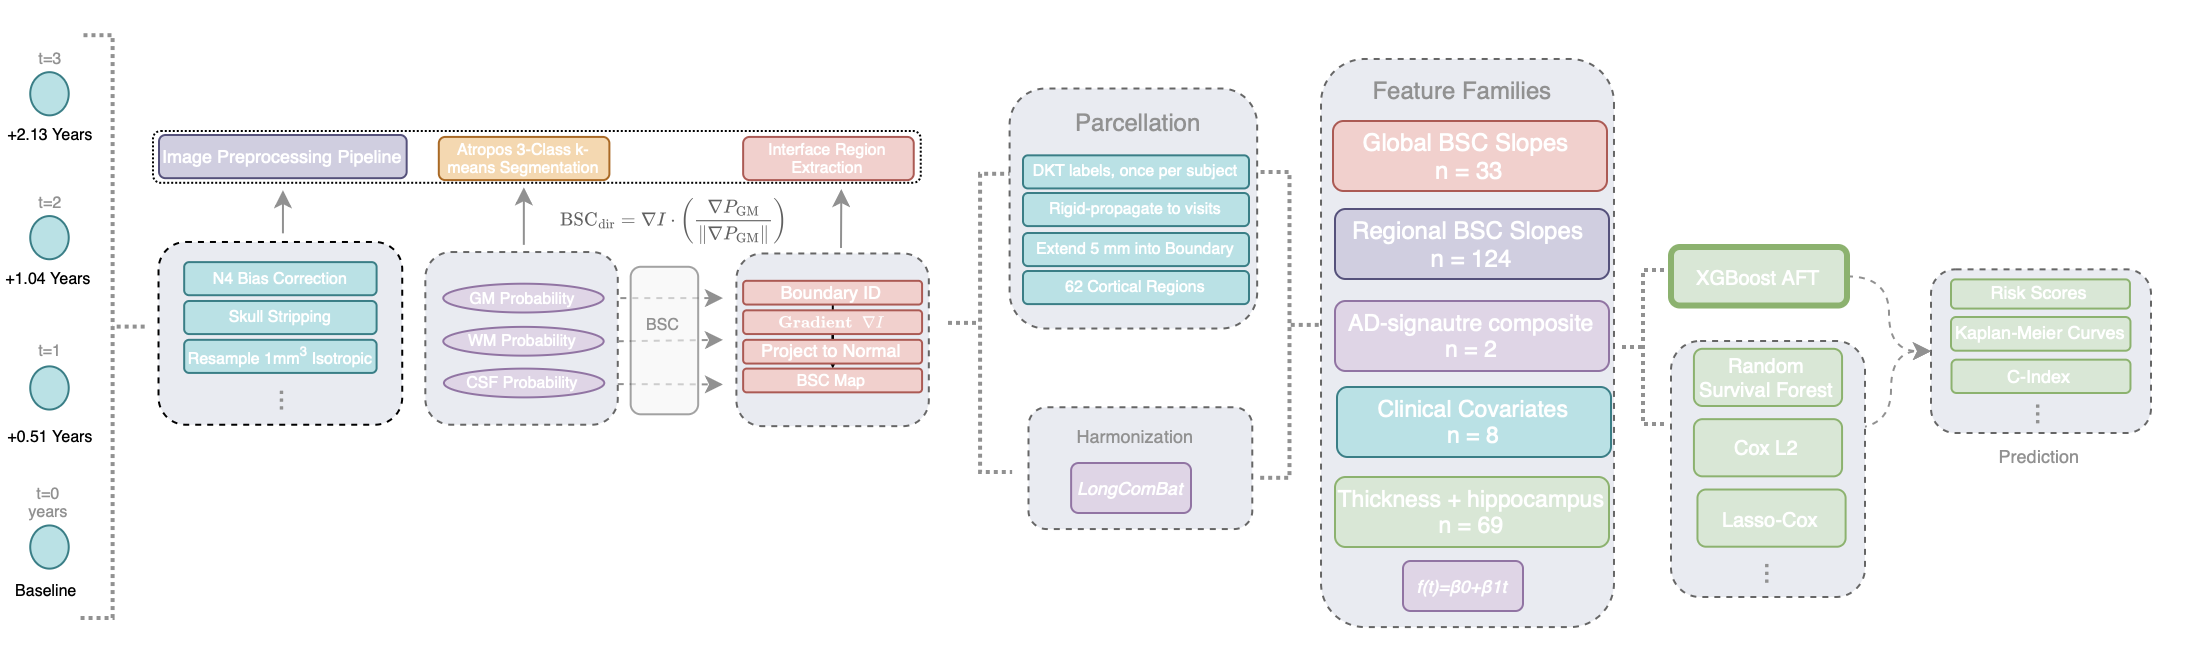
\includegraphics[width=\textwidth]{fig2.png}
\caption{Analysis pipeline. Numbered stages read left to right. Acquisition
dates are taken from the image archive rather than inferred from nominal visit
labels, and every scan acquired at or after the dementia diagnosis is excluded,
with the survival clock starting at the last remaining scan. Per-scan features
are harmonized across scanners and a cortical parcellation branch produces
regional measures. Clinical covariates and the FreeSurfer comparator measures
enter from ADNI tables without passing through the imaging pipeline, which is
what allows the incremental value of BSC to be tested against them. Stages 10 to
12 branch off the main sequence and are numbered by where they branch. Stage 10
leaves the BSC map, because construct validity asks what the measure tracks
rather than what it predicts, and it works from the per-scan maps rather than
from the fitted models. Stages 11 and 12 leave evaluation, because both re-fit
the stage 8 models on the frozen cross-validation folds, one under a competing-risk
coding of the outcome and one in the amyloid-confirmed subsample. Stages 11 and
12 also draw on ADNI registry, adverse-event and biomarker tables that the
imaging pipeline never touches.}
\label{fig:arch}
\end{figure*}

\subsection{Image processing and BSC computation}

Figure~\ref{fig:arch} summarizes the analysis pipeline. ADNI participants underwent T1-weighted structural MRI on 1.5T or 3T scanners using standardized protocols~\cite{jack2008adni_mri}, typically 3D MPRAGE with TR = 2300 ms, TE = 2.98 ms, TI = 900 ms, flip angle 9$^\circ$ and 1 mm isotropic voxels.

Preprocessing applied N4 bias correction~\cite{tustison2010n4} to reduce low-frequency intensity non-uniformity, since gradual brightness shifts could otherwise be mistaken for boundary change. Skull stripping used Otsu thresholding with morphological cleanup. Images were resampled to 1 mm$^3$ isotropic resolution with linear interpolation, chosen because higher-order interpolation can introduce ringing that would contaminate later gradient computation. Tissue segmentation used Atropos $k$-means clustering~\cite{avants2011atropos} with three classes. Gradients were estimated with 3D Gaussian derivative filters at $\sigma = 1.0$ mm.

BSC computation followed a multi-step pipeline. Atropos $k$-means clustering~\cite{avants2011atropos} assigned each voxel a probability of belonging to gray matter, white matter or cerebrospinal fluid. Boundary voxels were defined as those where gray matter probability fell between 0.4 and 0.6, which captures a transition band rather than forcing the analysis onto an unstable single-voxel contour. Gradient filters then measured how rapidly intensity changed across that boundary, projected along the direction perpendicular to the interface. For each boundary voxel $\mathbf{x}$, the directional BSC was computed as

\begin{equation}
    \text{BSC}_{\text{dir}}(\mathbf{x}) = \nabla I(\mathbf{x}) \cdot \frac{\nabla P_{GM}(\mathbf{x})}{\|\nabla P_{GM}(\mathbf{x})\|}
\end{equation}

where $I(\mathbf{x})$ is MRI intensity and $P_{GM}$ the gray matter probability map. The dot product isolates the component of the intensity gradient aligned with the boundary normal. Positive values indicate the expected increase in intensity moving from gray matter toward white matter.

Scanner metadata were extracted for every scan from the ADNI image archive, giving field strength, manufacturer, scanner model and acquisition site. Field strength was recovered for all scans and vendor for 97\%. Acquisition dates were also recovered from the archive, since the de-identified image files themselves carry no absolute date. This mattered more than expected: dates previously inferred from nominal visit labels differed from true acquisition dates by a median of 21 days and by more than 90 days for 7\% of scans, and slopes are regressed against this time axis. Real dates were matched for 96.4\% of scans; the remainder retain the nominal estimate.

\subsection{Scanner harmonization}

Longitudinal ComBat~\cite{beer2020longitudinal} was applied to the per-scan BSC features. Standard ComBat assumes independent observations, which is wrong here, since each subject contributes several scans and the within-subject correlation is the quantity of interest. The longitudinal variant adds a subject random intercept so that batch effects are estimated after accounting for repeated measures. Batch effects were estimated as fixed effects jointly with that random intercept, because estimating the intercept first and reading batch off the residuals biases the batch effect toward zero for subjects scanned entirely on one scanner. Batch parameters were shrunk toward their across-feature means by empirical Bayes.

The definition of a batch turned out to matter more than the harmonization itself. Candidate definitions were compared by how much each reduced the within-subject step in BSC observed when a subject changes scanner mid-study, which is a within-subject quantity and therefore free of between-subject confounding. Harmonizing on field strength alone did not help at all, changing the step by $-1.8\%$, and vendor combined with field strength performed no better at $-1.9\%$. Only definitions including acquisition site helped, with site combined with vendor and field strength reducing the step by 24.7\% across 124 batches. That definition was used throughout.

Two features of this result deserve emphasis. First, the group-level difference between 1.5T and 3T scans is small (Cohen's $|d| = 0.09$), because the direction of the step varies between scanner pairs and averaging across subjects cancels much of it. A group comparison on field strength therefore understates the problem substantially. Second, harmonization removes roughly a quarter of the within-subject step, not all of it. Residual scanner variance remains, and the field-strength issue should not be considered resolved.


\subsection{Feature construction}

For each scan, 33 BSC summary features were extracted (Table~\ref{tab:bsc-features}), covering boundary voxel count, directional and magnitude summary statistics, percentiles and spatial bin summaries. Each feature was regressed against time within subject:

\begin{equation}
    f_s(t) = \beta_0 + \beta_1 \cdot t + \epsilon
\end{equation}

where $\beta_1$ is the annualized rate of change. Slopes were computed on harmonized features, using real acquisition dates, and only over scans acquired while the subject was still MCI.

\begin{table}[htbp]
\centering
\caption{BSC feature categories extracted per scan}
\label{tab:bsc-features}
\begin{tabular}{lc}
\hline
\textbf{Feature Category} & \textbf{Count} \\
\hline
Boundary count (Nboundary) & 1 \\
Directional statistics (mean, std, median) & 3 \\
Directional percentiles (p10, p25, p50, p75, p90) & 5 \\
Magnitude statistics (mean, std, median) & 3 \\
Magnitude percentiles (p10, p25, p50, p75, p90) & 5 \\
Directional spatial bins (8 bins) & 8 \\
Magnitude spatial bins (8 bins) & 8 \\
\hline
\textbf{Total per scan} & \textbf{33} \\
\hline
\end{tabular}
\end{table}

For each base feature, four longitudinal descriptors were derived: baseline value, final value, annual slope and goodness of fit ($R^2$).

Raw slope features showed extreme heterogeneity in variance, with the boundary count slope varying on a far larger scale than the rest. Selection and preprocessing were carried out on training folds only. Slope values were transformed with a signed logarithm, $\text{sign}(x) \cdot \log(1 + |x|)$, which compresses extreme values while preserving direction. Outliers were then clipped by winsorization~\cite{tukey1962future} at the 1st and 99th percentiles, followed by MinMax scaling to $[0, 1]$. A 0.10 penalty factor was applied to boundary count features during variance ranking only, which altered ranking scores rather than the values used for modeling. Models that perform their own selection, including the gradient-boosted and penalized regression models, received the full feature set.

Global summaries collapse the whole cortex into a single number, which discards the regional specificity that AD pathology is known to have. BSC was therefore computed within cortical parcels.

Labels came from the Desikan-Killiany-Tourville protocol, generated with a deep learning parcellation~\cite{tustison2021antsxnet} applied to the T1 volume directly, which avoids the cost of full surface reconstruction. Since the quantity of interest is a slope, generating labels independently at each visit would inject parcellation noise straight into the modeled quantity. Labels were therefore generated once per subject and propagated to that subject's other timepoints by rigid registration, which is adequate within subject and avoids deforming the cortical ribbon. The reference scan was chosen by quality control rather than assumed to be the baseline, since parcellation failed outright on 13.7\% of baseline scans and a failed reference propagates to every timepoint for that subject.

One adjustment was necessary. The parcellation labels the cortical gray ribbon, whereas the BSC boundary band sits at the gray-white interface and therefore falls largely in unlabeled white matter. Intersecting the two directly captured under 10\% of boundary voxels and left region means resting on a median of 32 voxels. Each parcel was therefore extended inward to its nearest boundary voxels using a Euclidean distance transform, with assignment refused beyond 5 mm so that deep white matter is not attributed to a parcel it does not border. This raised the median to 185 voxels per region. Coverage plateaus near 50\% of the boundary band because the band also spans cerebellar, subcortical and ventricular interfaces that have no cortical parcel.

The analysis retained 62 cortical parcels. Each parcel yielded a directional and a magnitude slope, giving 124 regional features; with the 33 global slopes and the two composite features, the full pool screened univariately contained 159 slopes. In addition, a single AD-signature composite was specified in advance as the voxel-weighted mean across seven bilateral regions selected from the AD literature: entorhinal cortex, parahippocampal gyrus, inferior temporal cortex, middle temporal cortex, precuneus, posterior cingulate and fusiform gyrus. The composite was computed separately for directional and magnitude BSC, giving two features. Specifying it before analysis gives one biologically motivated test that does not depend on selection among 62 regions.

Eight covariates were drawn from ADNI clinical tables at the landmark visit: age, sex, years of education, APOE4 allele count, MMSE, ADAS-Cog13, CDR sum of boxes, and field strength. Missingness was low, affecting 6 subjects for MMSE, 7 for ADAS-Cog13 and 15 for CDR sum of boxes, with none missing for the remaining covariates. Missing values were imputed with the training-fold median.

To test whether BSC adds anything to established longitudinal MRI, cortical thickness was extracted for 68 Desikan-Killiany regions and hippocampal volume normalized by intracranial volume from the ADNI FreeSurfer tables, matched to each scan by subject and examination date within 120 days. Slopes were computed over the identical windows and with the identical procedure used for BSC, so the two feature families differ in what they measure rather than in how they are summarized.

\subsection{Survival analysis}

For each subject, $t_{\text{last}}$ is the date of the last MRI used in feature computation, which for converters is the last scan preceding the dementia diagnosis. The event date is the date of first dementia diagnosis taken from the clinical record rather than from a scan label, and censoring is at last known clinical follow-up. Time to event is $(t_{\text{event}} - t_{\text{last}})/365.25$ in years. As noted in the inclusion criteria, only subjects with positive time were retained.

Taking conversion dates from the clinical record rather than from scan diagnoses matters, because a subject whose conversion is recorded at a clinic visit between two scans would otherwise be dated to the later scan.

Seven models were fitted. The primary model was gradient-boosted survival regression with an accelerated failure time objective~\cite{barnwal2022survivalxgb}, which accommodates nonlinear structure and performs its own feature selection. Comparators were Random Survival Forest~\cite{ishwaran2008rsf} with 1,000 trees, Cox proportional hazards~\cite{cox1972} with L2 penalization, Lasso-penalized Cox, and Weibull, log-normal and log-logistic accelerated failure time models with penalizer 0.1. Including both a penalized Cox model and all three parametric AFT families allows the reader to see whether conclusions depend on model family, which they largely do not.

Given the modest event count, performance was estimated by stratified 5-fold cross-validation rather than a single split, and is reported as mean and standard deviation across folds. A 20\% stratified hold-out was reserved, never used during model development, and evaluated once. All imputation, transformation, winsorization and scaling parameters were estimated within training folds and applied to held-out folds.

Discrimination was measured by Harrell's concordance index and by Uno's inverse-probability-weighted concordance index~\cite{uno2011cstat}, which is better behaved under censoring. Time-dependent AUC was computed at one, two and three years.

A single convention was applied: a higher risk score corresponds to shorter time to conversion. After fitting, the concordance between predicted risk and observed time was evaluated \textit{on the training fold}, and the risk score was negated if that concordance fell below 0.5. Accelerated failure time models predict survival time rather than risk, so their predictions are negated by construction.

Determining the direction on training data only is deliberate. Choosing the sign that makes held-out performance look better would guarantee a C-index above 0.5 for any model, including a model with no signal, and would make the metric uninterpretable. A consequence is that genuinely uninformative feature sets can and do produce held-out values below 0.5, and these are reported as they are.

The question of whether BSC adds information is a nested comparison, and comparing two marginal cross-validation means does not answer it. Each pair of feature sets was therefore refitted on identical folds, the per-fold difference in C-index was taken, and a 95\% interval was obtained by resampling subjects from the pooled out-of-fold predictions. Nested Cox models were additionally compared by likelihood ratio test. Individual slopes were screened univariately with Benjamini-Hochberg control of the false discovery rate.

Conversion is observed at scheduled clinic visits rather than on the day it occurs, so the outcome is strictly interval-censored, and Zhang et al.~\cite{zhang2024interval} model it that way. Right-censored models were used here regardless. ADNI schedules visits every six to twelve months over a median follow-up of 1.04 years, so the interval containing each conversion is short relative to the spread of conversion times, and the right-censored approximation is adequate at that visit density. It would not be adequate in a cohort seen every three years.

Calibration was assessed as well as discrimination, since a claim that clinical covariates are sufficient is stronger if they are also well calibrated. The integrated Brier score was computed over the first three years for the covariates-only, covariates-plus-standard-MRI and full models, alongside the Brier score and time-dependent AUC at one, two and three years. Brier scores need a predicted survival function rather than a risk score, so they were computed for the penalized Cox and Random Survival Forest fits. The gradient-boosted AFT model returns a predicted time, and constructing a survival curve for it would be a modelling choice reported as a measurement.

To isolate the effect of the follow-up definition, the cohort was also rebuilt under the original design, in which features come from every scan including those acquired after diagnosis and the clock starts at the MCI baseline scan. Both designs were then restricted to the subjects present in each, so that the same people, features and models are compared and only the timing differs. The mechanism at work in the looser design is guarantee-time bias: a subject cannot enter the analysis until enough scans have accumulated, so surviving long enough to be scanned repeatedly is a precondition for inclusion, and features measured over that guaranteed interval carry information about an outcome that has in part already occurred.

\subsection{Competing risks}

The cohort has a mean age of 76.9 years at the landmark and multi-year follow-up, so death is a competing event rather than a nuisance, and treating it as ordinary censoring assumes that a subject who dies would have gone on to convert at the same rate as one still under observation.

Death was ascertained from two ADNI tables, which between them cover the whole study but not in the same format. TREATDIS records a reason for withdrawal with an exact form date and covers ADNI1, ADNIGO and ADNI2; the code for death is 2 in the ADNI1 data dictionary and 1 in every later one, and was mapped per protocol. ADVERSE records a date of death in the field AEHDTHDT and covers ADNI3 and ADNI4, but that field is de-identified to a year, so those deaths were placed at the midpoint of the year reported. No cohort subject appears in both tables.

Deaths in this cohort are recorded after the last clinical visit rather than during observation, by a median of 0.95 years. A subject known to have died without a dementia diagnosis was therefore followed to the death date and treated as having experienced the competing event there. Death recorded after a dementia diagnosis is not a competing event, since the outcome of interest had already occurred.

Three configurations were refitted under this coding: clinical covariates alone, regional BSC slopes alone, and the full set of covariates with regional BSC and standard MRI. Two framings are reported. The cause-specific framing censors the competing event and reports how many there are. The Fine-Gray subdistribution hazard~\cite{fine1999proportional} was fitted to the out-of-fold risk score of each configuration using Geskus's weighted Cox formulation~\cite{geskus2011cause}, in which subjects who experience the competing event remain in the risk set afterwards carrying the time-varying weight $G(t)/G(T_i)$, where $G$ is the Kaplan-Meier estimate of the censoring distribution. Confidence intervals come from resampling subjects 400 times, because the weights are estimated and the naive partial-likelihood standard error does not account for that. Unlike the models in Table~\ref{tab:model-performance}, these use all 417 subjects in cross-validation with no hold-out reserved, so their baseline column is recomputed rather than copied across.

\subsection{Biomarker-confirmed subgroup}

The outcome is a diagnosis code, not a biologically confirmed one, so the whole analysis was repeated in the subjects with confirmed amyloid pathology. Amyloid status was taken from the measurement closest to and no later than the landmark visit, with a 180 day grace window because ADNI schedules PET and lumbar puncture near rather than on the clinical visit. Nothing acquired after the landmark was used, since a scan ordered after a subject converted would carry the outcome into the predictor. Amyloid PET was preferred where available and CSF A$\beta$42 from the Roche Elecsys assay was the fallback, dichotomized at the ADNI reference cutoff of 977 pg/mL. Where both existed they agreed for 84\% of 249 subjects. Tau PET was attached where available but is too sparse to stratify on, and is used below only for construct validity.

Two analyses follow from this. The incremental-value tests were rerun inside the amyloid-positive subgroup, where every subject has confirmed pathology. They were also rerun on the full cohort with amyloid status entered into the baseline block as a positivity flag plus an indicator for untested, which keeps all 417 subjects without imputing a status that is missing for reasons connected to the outcome.

\subsection{Construct validity and scanner signal}

What BSC measures is a separate question from whether it predicts, and four analyses beyond the cross-sectional correlations were run to answer it.

The first is a within-subject analysis. A correlation computed across scans cannot separate a property of the measure from a property of the people being measured, since a subject who is scanned on a noisier machine may also differ in ways that have nothing to do with the machine. For the 412 subjects with three or more scans, every variable was standardized and then centred on that subject's own mean, which removes every time-invariant subject characteristic by construction. The centred data were fitted by least squares with standard errors clustered on subject, giving the within-subject estimate. A mixed model with a subject random intercept was fitted to the uncentred scans as a check, and a regression on the subject means gives the between-subject contrast. Centring removes the subject intercept, so no random intercept is fitted on top of the centred data: the variance component would sit on the boundary at zero.

The second is a partial association. The association between BSC and conversion was estimated before and after the image-quality slopes were partialled out, as a Cox hazard ratio per standard deviation. This was done both for the global BSC slope and for the out-of-fold risk score of the regional feature set, since it is the regional set that reaches a C-index of 0.649 and therefore the regional score that the question is really about.

The third is a scanner-signal test with two parts. A survival model was given nothing but acquisition structure: indicators for site, vendor and field strength, with sites contributing fewer than ten subjects pooled, since a dummy variable fitted to three subjects encodes those subjects rather than their scanner. This gives 12 site indicators, three vendor indicators and field strength. If acquisition structure alone discriminates converters, that quantifies how much outcome information the design carries. Then each regional BSC feature was residualized on the same design matrix, with the residualizing regression fitted on training rows only, and the regional model refitted on the residuals. A large drop would show that the 0.649 was partly acquisition signal.

BSC slopes were also correlated against amyloid PET centiloids, CSF A$\beta$42, CSF p-tau, the CSF p-tau to A$\beta$42 ratio and tau PET meta-temporal SUVR, with Benjamini-Hochberg control across all 159 slopes for each target. A marker of Alzheimer's pathology should track at least one of these.

\subsection{Software and reproducibility}

Analyses were conducted in Python 3.12. Preprocessing used Advanced Normalization Tools~\cite{avants2011ants}, cortical parcellation used ANTsXNet~\cite{tustison2021antsxnet}, survival modeling used scikit-survival~\cite{polsterl2020sksurv}, lifelines~\cite{davidson-pilon2019lifelines} and XGBoost~\cite{chen2016xgboost}, and the mixed models used statsmodels. The Fine-Gray fit uses the weighted Cox formulation implemented over lifelines rather than a packaged subdistribution routine, since no maintained Python implementation covers it. Longitudinal ComBat was implemented directly following Beer et al.~\cite{beer2020longitudinal}. Code is publicly available at \texttt{github.com/ishaan-cherukuri/research/tree/main/mri-bsc}.

\section{Results}

\subsection{Cohort characteristics}


Table~\ref{tab:demographics} summarizes the corrected cohort. Converters and stable subjects did not differ detectably in age, sex or education, but differed on every cognitive measure and on APOE4 carriage, as expected.

Two entries deserve comment because they shape the interpretation of everything that follows. Half of converters were scanned at 3T at the landmark visit compared with three quarters of stable subjects ($p<0.001$), so field strength is confounded with the outcome and any residual scanner effect is correlated with the label rather than being noise. Converters also contributed fewer scans over shorter windows, which is a direct consequence of requiring scans to precede conversion.

\subsection{Survival model performance}

\begin{table*}[t!]
\centering
\caption{Cross-validated C-index by feature set and model family. Values are means across five stratified folds. Feature counts are given in parentheses. The Lasso-Cox column repeats across the combined feature sets because the penalty shrinks the imaging coefficients to zero, leaving essentially the same covariate model in each case.}
\label{tab:model-performance}
\begin{tabular}{lccccccc}
\hline
\textbf{Feature set} & \textbf{XGB AFT} & \textbf{RSF} & \textbf{Cox L2} & \textbf{Cox Lasso} & \textbf{Weibull} & \textbf{LogNorm} & \textbf{LogLog} \\
\hline
Clinical covariates (8) & 0.773 & 0.778 & 0.793 & 0.788 & 0.795 & 0.789 & 0.789 \\
BSC baseline (33) & 0.472 & 0.444 & 0.520 & 0.494 & 0.510 & 0.528 & 0.532 \\
BSC slopes, global (33) & 0.540 & 0.584 & 0.443 & 0.391 & 0.422 & 0.428 & 0.425 \\
BSC slopes, regional (124) & 0.642 & 0.649 & 0.511 & 0.514 & 0.512 & 0.536 & 0.529 \\
AD-signature composite (2) & 0.512 & 0.546 & 0.409 & 0.454 & 0.432 & 0.433 & 0.430 \\
Thickness + hippocampus (69) & 0.685 & 0.711 & 0.527 & 0.559 & 0.543 & 0.548 & 0.547 \\
\hline
Covariates + BSC global (41) & 0.788 & 0.754 & 0.769 & 0.788 & 0.765 & 0.773 & 0.771 \\
Covariates + BSC regional (132) & 0.788 & 0.762 & 0.695 & 0.788 & 0.694 & 0.714 & 0.721 \\
Covariates + AD-signature (10) & 0.790 & 0.782 & 0.775 & 0.788 & 0.777 & 0.779 & 0.776 \\
Covariates + standard MRI (77) & 0.778 & 0.779 & 0.698 & 0.783 & 0.706 & 0.715 & 0.718 \\
Covariates + BSC + standard MRI (110) & 0.778 & 0.763 & 0.715 & 0.783 & 0.708 & 0.718 & 0.711 \\
Covariates + regional + standard MRI (201) & 0.796 & 0.762 & 0.688 & 0.782 & 0.669 & 0.666 & 0.667 \\
\hline
\end{tabular}
\end{table*}

Table~\ref{tab:model-performance} reports all seven model families across all feature sets, and Figure~\ref{fig:models} shows how far each feature set moves across those families. Clinical covariates alone reached 0.773 to 0.795 depending on model family and were the strongest single block in the study. Global BSC slopes reached 0.584 at best, with a Random Survival Forest, and fell below chance in five of the seven families. Regional BSC slopes reached 0.649, clearly better than the global summaries they replace. Longitudinal cortical thickness and hippocampal volume reached 0.711.

The gap between training and held-out folds separates the two kinds of feature set more sharply than the held-out value does. Averaged over folds, the covariate models lost 0.017 (Weibull) and 0.025 (Cox L2) between training and test, while every imaging configuration lost an order of magnitude more: 0.173 for thickness with hippocampal volume, 0.199 for global BSC slopes, 0.206 for regional BSC slopes and 0.212 for the full combined model, which trained to 0.984 against a test value of 0.772.

Uno's concordance index gave the same ordering, with the flagship model at 0.772 for covariates, 0.529 for global BSC slopes and 0.644 for regional slopes. The hold-out set contained 84 subjects and 27 events, which is too few to support a precise estimate, and hold-out values should be read as a consistency check rather than as headline performance.

Time-dependent AUC for the flagship model rose with the horizon, reaching 0.777, 0.816 and 0.857 at one, two and three years for clinical covariates, against 0.641, 0.701 and 0.669 for regional BSC slopes. The ordering matches the C-index at every horizon.

Calibration tells the same story more sharply, because it can get worse when discrimination does not. The integrated Brier score over the first three years was lowest for clinical covariates alone in both model families that produce a survival function: 0.142 against 0.152 for covariates with standard MRI and 0.161 for the full set under penalized Cox, and 0.138 against 0.141 and 0.144 under a Random Survival Forest. Adding imaging to the covariate model did not improve calibration in any comparison, and under the Cox model it degraded it. A covariate-only model is therefore not merely as discriminating as the imaging models but better calibrated than any of them.

Figure~\ref{fig:km} shows the same contrast as survival curves: stratifying by clinical covariates separates the risk tertiles widely, while stratifying by regional BSC slopes separates them far less. Thirteen of the 91 model and feature-set combinations produced cross-validated values below 0.5, concentrated in the BSC-only and AD-signature-only sets. Because the risk direction was fixed on training folds, these are genuine indications that the feature set carries no usable signal in held-out data rather than reversed scores. Reporting them as values above 0.5 would require choosing the sign from test performance, which would make the metric meaningless.


\begin{figure*}[t!]
\centering
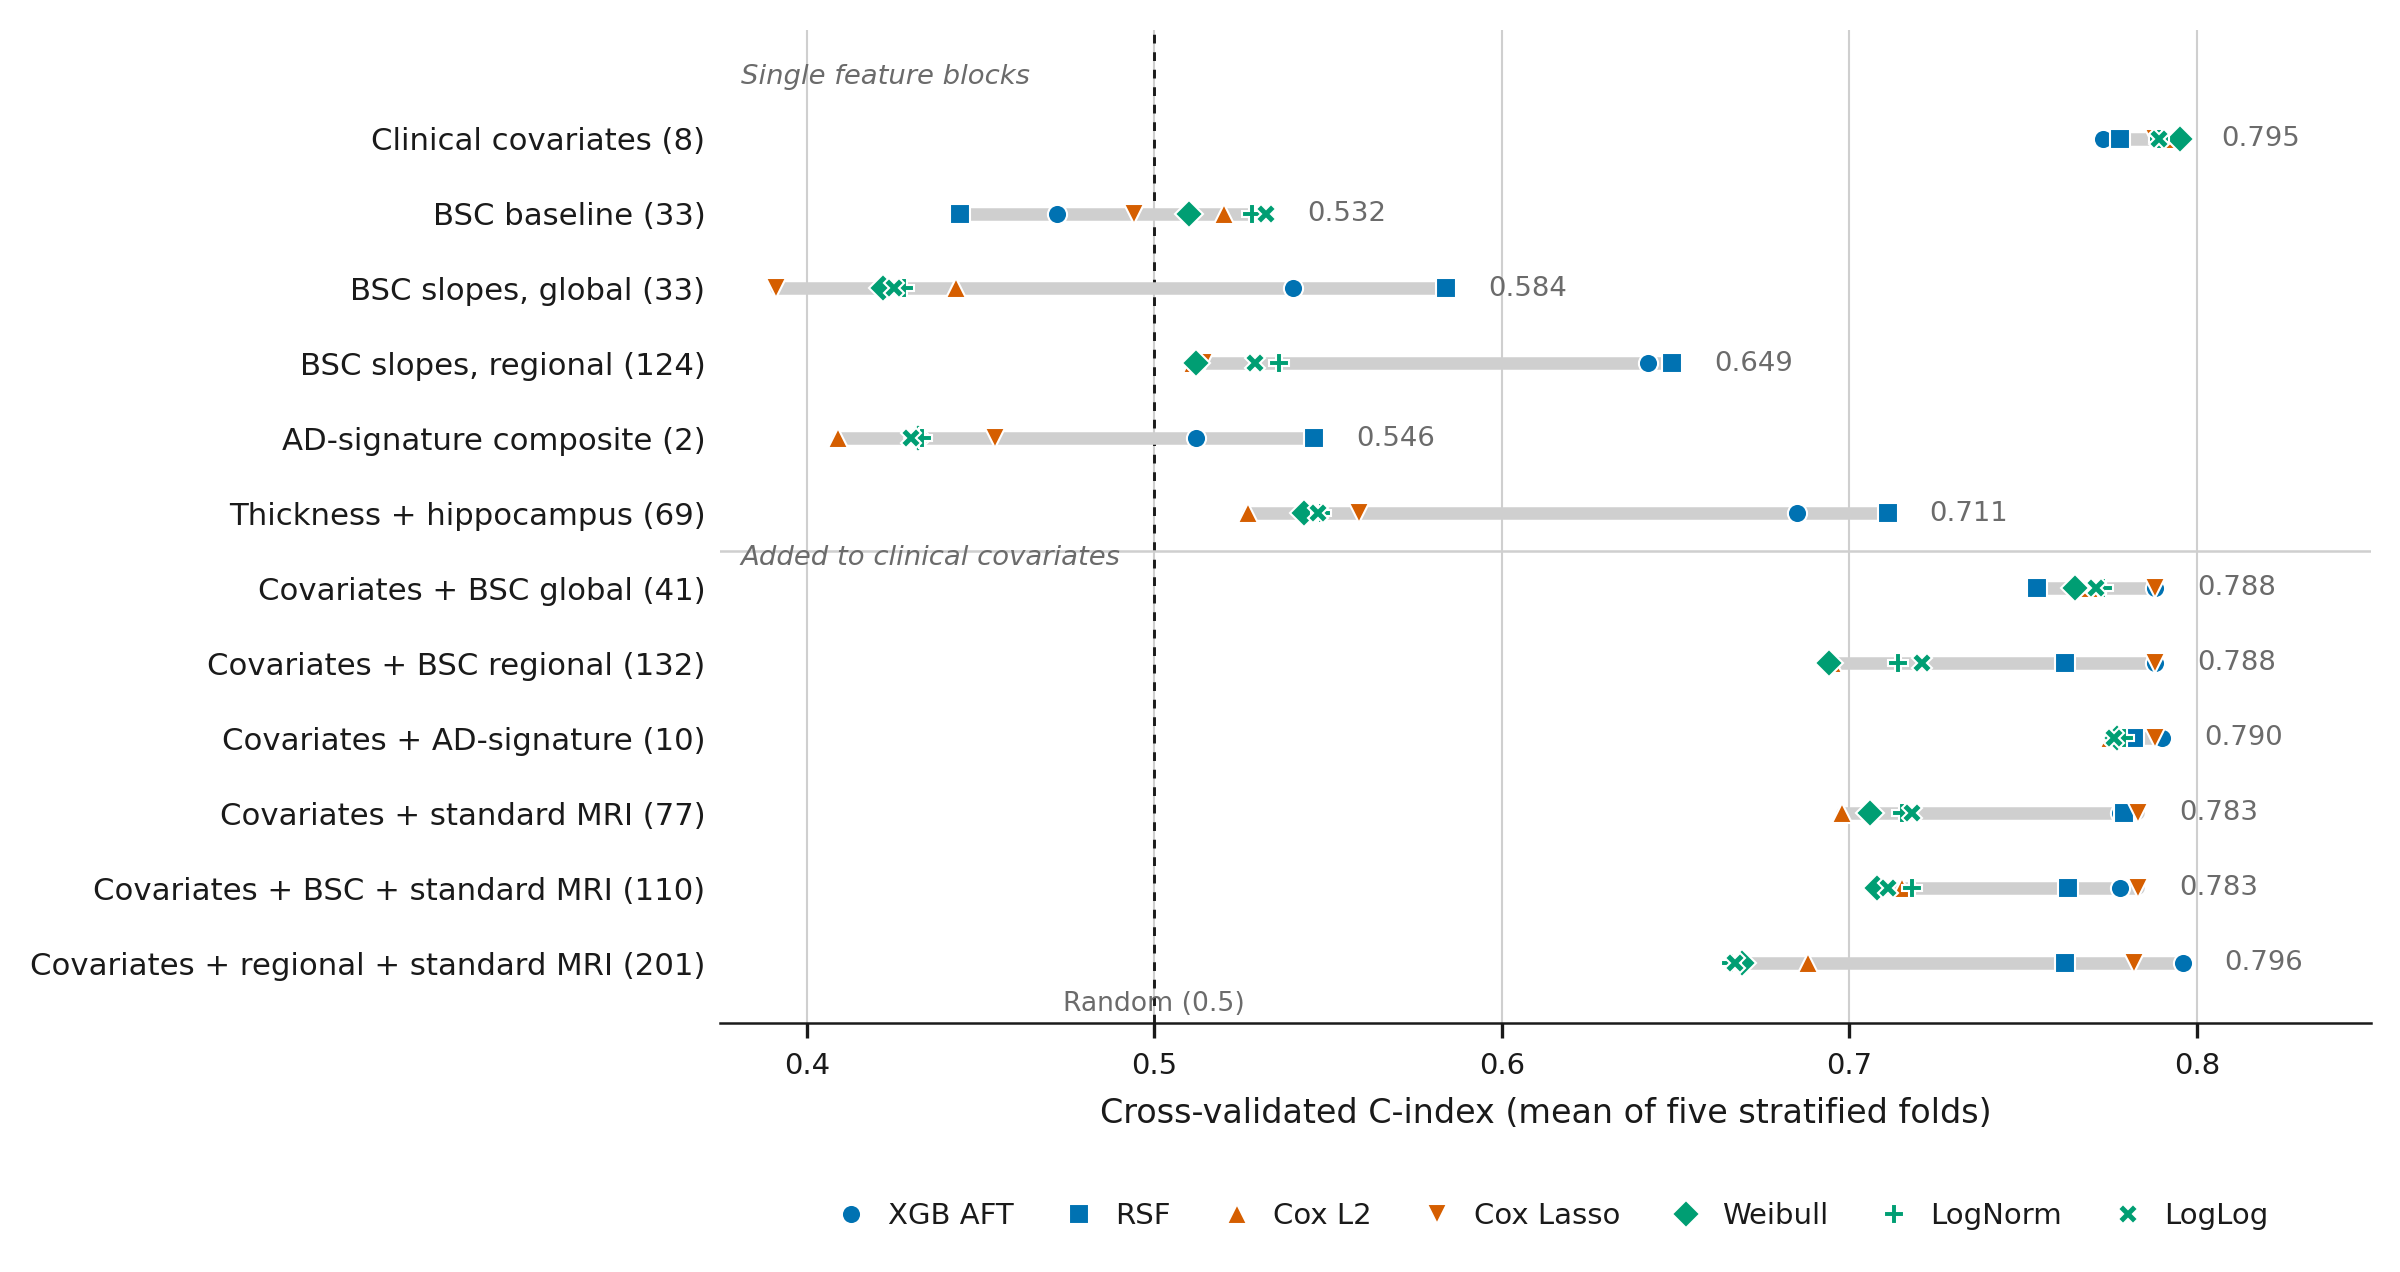
\includegraphics[width=\textwidth]{fig3.png}
\caption{Cross-validated C-index for every feature set against every model
family. One row per feature set with the number of features in parentheses, one
marker per family, and a connector spanning the range across families, which
separates what the feature set contributes from what the fitter contributes. The
figure to the right of each row is the best value across families. Clinical
covariates sit above every imaging block and vary little across families, whereas
the BSC-only blocks span as much as 0.19 of C-index depending on which model is
fitted and fall below chance in several of them. Values are means over five stratified
folds, and the risk direction is fixed on training folds, so a value below 0.5
records a feature set carrying no usable signal rather than a reversed score.}
\label{fig:models}
\end{figure*}

\begin{figure*}[t!]
\centering
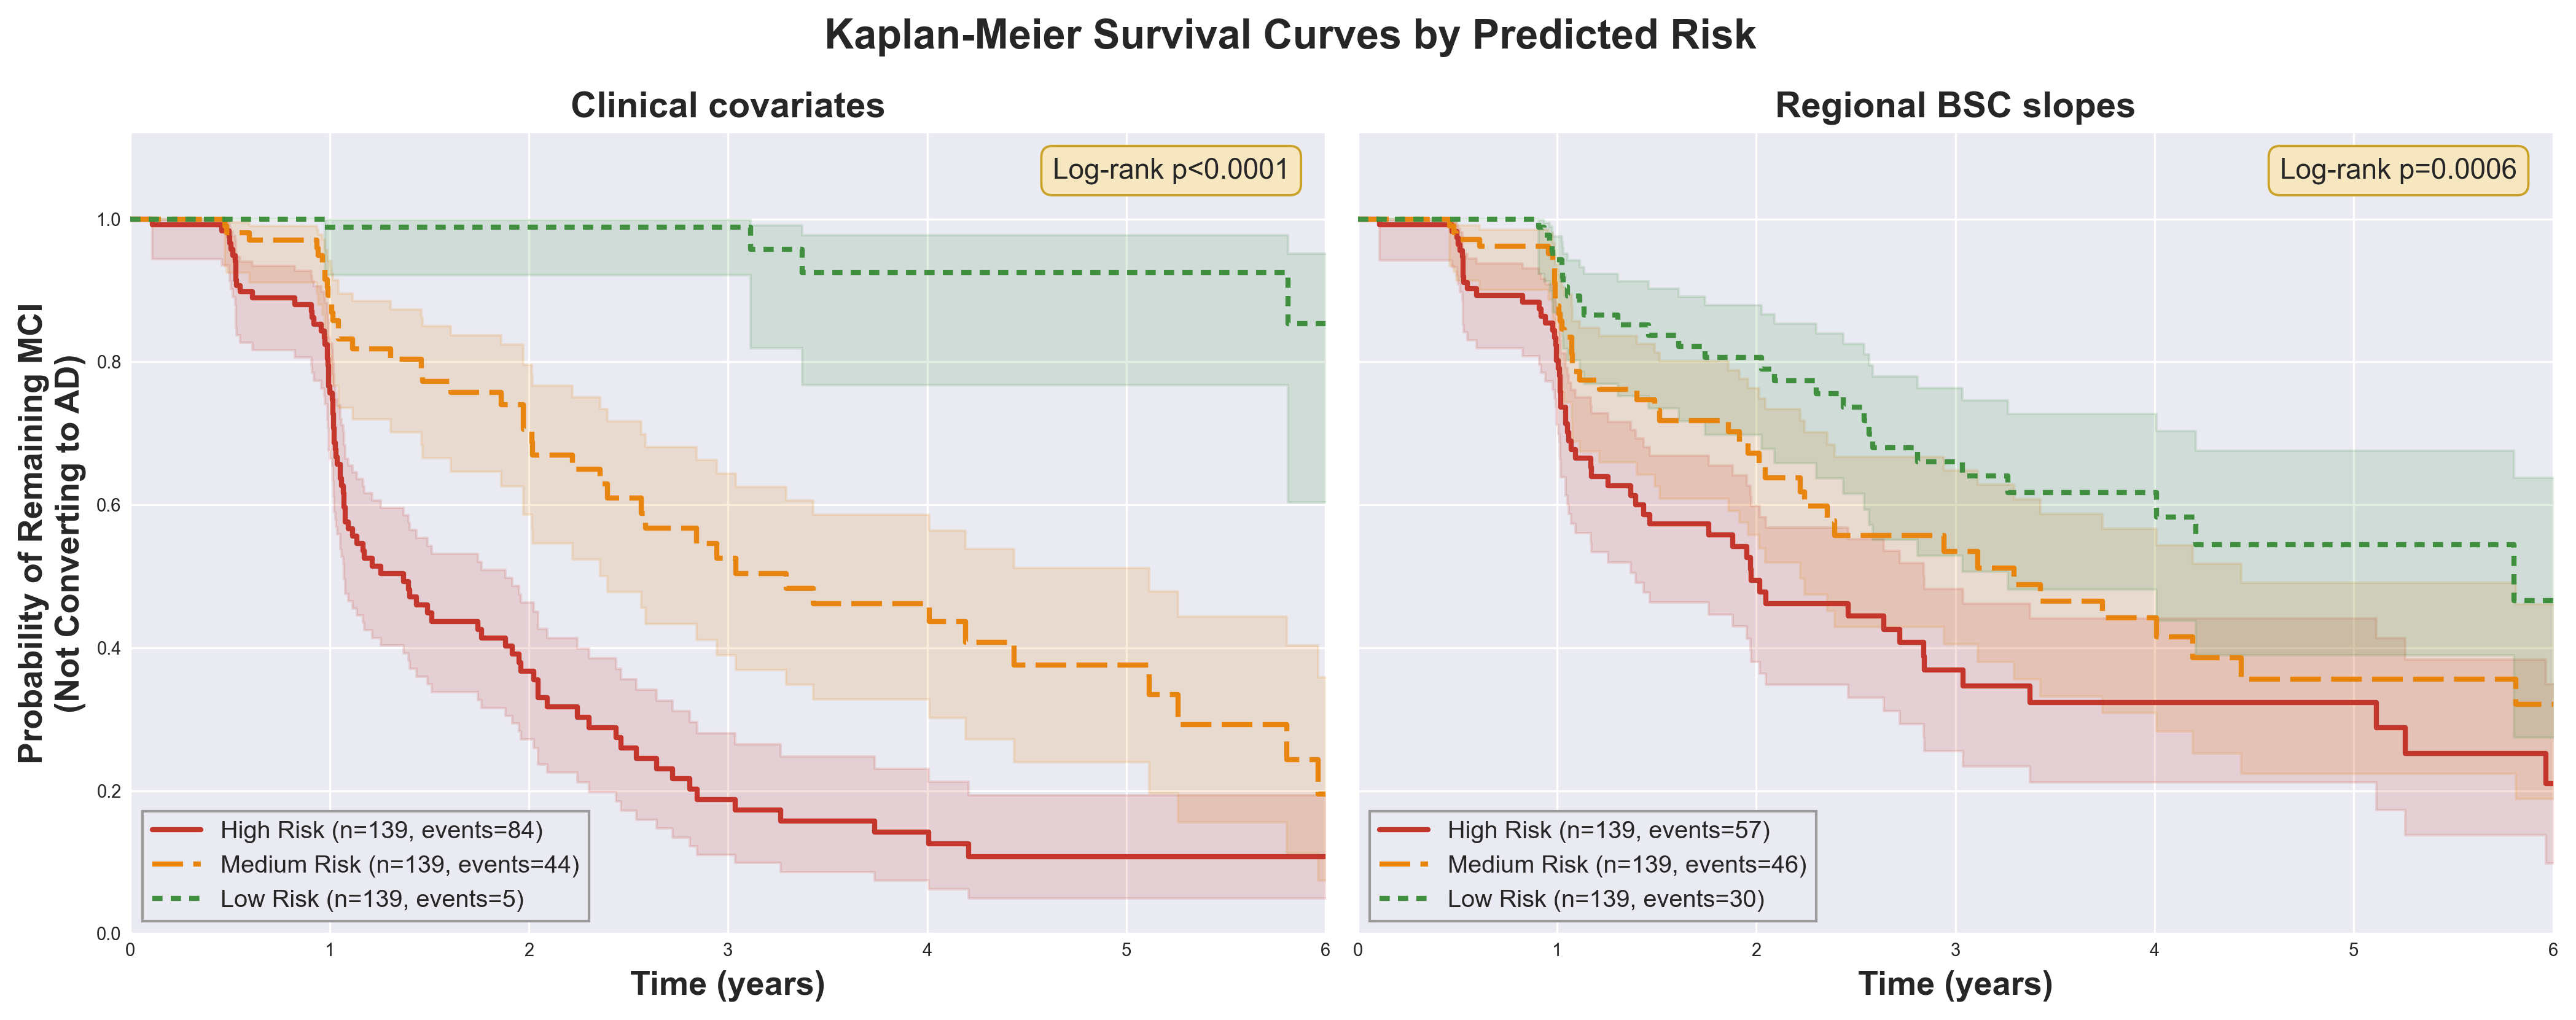
\includegraphics[width=\textwidth]{fig4.png}
\caption{Kaplan-Meier estimates of the probability of remaining MCI, stratified by tertile
of predicted risk. Risk scores are out-of-fold, so no subject is stratified by a model
fitted on them. Shaded bands are 95 per cent confidence intervals. Stratification by
clinical covariates separates the tertiles widely, with 5, 44 and 84 events.
Stratification by regional BSC slopes separates them far less, with 30, 46 and 57 events,
even though both log-rank tests are significant. The event counts are the more informative
comparison, since the log-rank test responds to any departure from equality rather than to
its size.}
\label{fig:km}
\end{figure*}

\subsection{Effect of the follow-up definition}

\begin{table*}[t!]
\centering
\caption{Cross-validated C-index under the original and corrected follow-up definitions, restricted to the 417 subjects present in both. Only the timing differs; subjects, features and models are identical.}
\label{tab:design}
\begin{tabular}{llccc}
\hline
\textbf{Feature set} & \textbf{Model} & \textbf{Original design} & \textbf{Corrected design} & \textbf{Change} \\
\hline
Clinical covariates & RSF & 0.786 & 0.775 & $-0.010$ \\
 & XGB AFT & 0.764 & 0.751 & $-0.013$ \\
 & Cox L2 & 0.804 & 0.769 & $-0.034$ \\
\hline
BSC slopes, global & RSF & 0.684 & 0.617 & $-0.066$ \\
 & XGB AFT & 0.616 & 0.587 & $-0.029$ \\
 & Cox L2 & 0.601 & 0.542 & $-0.059$ \\
\hline
BSC slopes, regional & RSF & 0.737 & 0.641 & $-0.096$ \\
 & XGB AFT & 0.656 & 0.615 & $-0.041$ \\
 & Cox L2 & 0.527 & 0.569 & $+0.042$ \\
\hline
Thickness + hippocampus & RSF & 0.781 & 0.685 & $-0.096$ \\
 & XGB AFT & 0.761 & 0.665 & $-0.096$ \\
 & Cox L2 & 0.647 & 0.570 & $-0.077$ \\
\hline
\end{tabular}
\end{table*}

Table~\ref{tab:design} and Figure~\ref{fig:design} isolate the effect of the follow-up definition. Under the original design the cohort contains 665 subjects with 293 converters and a median follow-up of 3.07 years. Under the corrected design it contains 417 subjects with 133 converters and a median follow-up of 1.04 years (mean 1.69, SD 1.86, as in Table~\ref{tab:demographics}). Restricting both to the 417 subjects present in each removes cohort composition as an explanation.

Clinical covariates lost between 0.010 and 0.034 in C-index when the design was corrected. Every imaging feature family lost substantially more. Global BSC slopes lost 0.029 to 0.132, regional BSC slopes lost up to 0.096, and cortical thickness with hippocampal volume lost 0.077 to 0.096 across all three model families.

The asymmetry is the result. A design in which features may be drawn from scans acquired after diagnosis inflates the apparent performance of longitudinal imaging markers while leaving clinical prediction close to unchanged. This is not specific to BSC. Standard volumetric measures, which are far better established, are affected as strongly. Under the original design, cortical thickness and hippocampal volume slopes reach 0.781 with a Random Survival Forest, which would be a strong result if it were real.


\begin{figure}[t!]
\centering
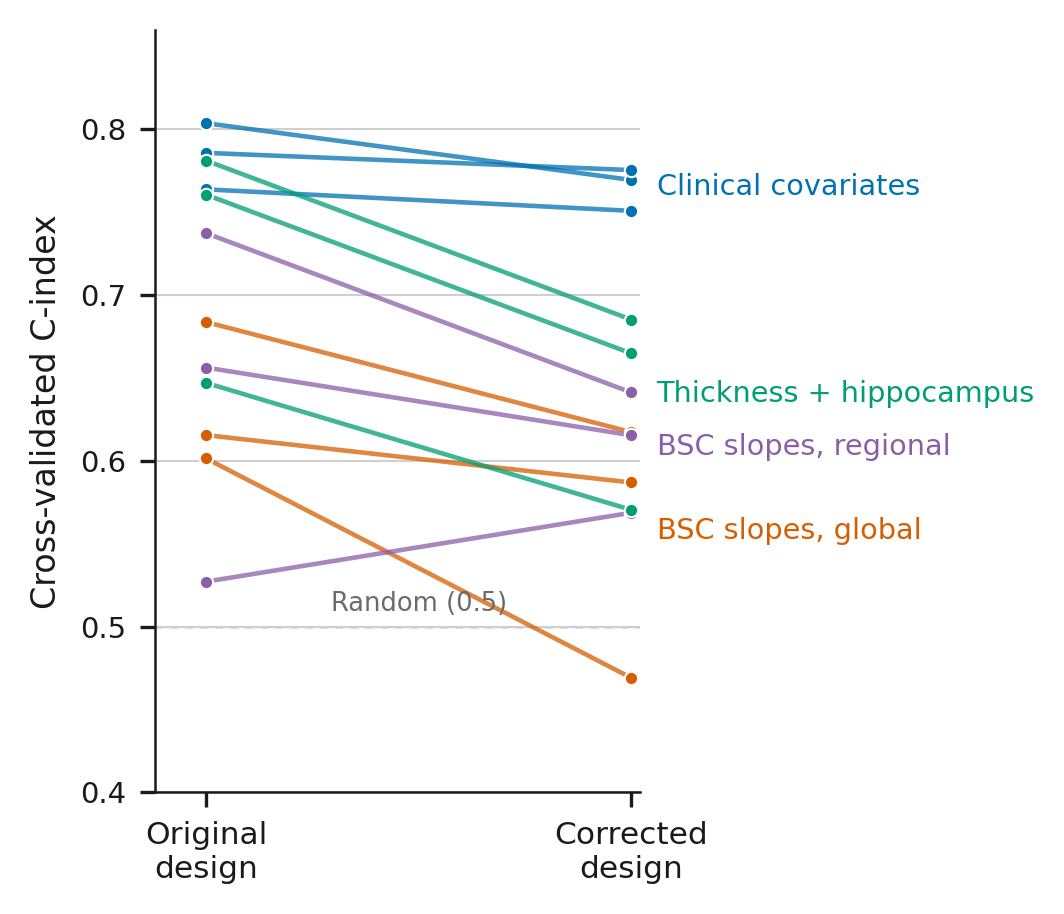
\includegraphics[width=\columnwidth]{fig5.png}
\caption{Effect of the follow-up definition, restricted to the 417 subjects present under
both designs so that only the timing differs. Each line is one model family fitted to one
feature set. Clinical covariates are close to flat, losing 0.010 to 0.034 in C-index.
Every imaging feature family falls substantially further, including cortical thickness
with hippocampal volume, which is an established measure rather than a novel one.}
\label{fig:design}
\end{figure}

\subsection{Incremental value of BSC}

\begin{table}[htbp]
\centering
\footnotesize
\setlength{\tabcolsep}{4pt}
\caption{Fold-matched incremental value, gradient-boosted AFT model. Intervals are 95\% bootstrap percentile intervals on the paired difference. Cov.\ denotes the eight clinical covariates and MRI denotes cortical thickness with hippocampal volume slopes.}
\label{tab:increment}
\begin{tabular}{lcc}
\hline
\textbf{Feature added} & \textbf{$\Delta$ C-index (95\% CI)} & \textbf{$p$} \\
\hline
\multicolumn{3}{l}{\textit{Baseline set: clinical covariates}} \\
\quad BSC global & $+0.022$ ($-0.001$, $+0.053$) & 1.00 \\
\quad BSC regional & $-0.000$ ($-0.032$, $+0.032$) & 1.00 \\
\quad AD-signature & $+0.011$ ($-0.016$, $+0.026$) & 0.85 \\
\quad Standard MRI & $+0.020$ ($-0.010$, $+0.049$) & 0.73 \\
\multicolumn{3}{l}{\textit{Baseline set: covariates + standard MRI}} \\
\quad BSC global & $-0.005$ ($-0.020$, $+0.012$) & 1.00 \\
\quad BSC regional & $+0.002$ ($-0.021$, $+0.022$) & 1.00 \\
\quad AD-signature & $+0.006$ ($-0.011$, $+0.017$) & 0.68 \\
\hline
\end{tabular}
\end{table}

Table~\ref{tab:increment} reports the nested comparisons. No BSC feature set improved on clinical covariates, and none improved on covariates combined with standard longitudinal MRI. Every interval includes zero, and every likelihood ratio test of the corresponding nested Cox models was non-significant.

Two entries need comment. Global BSC slopes over covariates gave the largest point estimate, $+0.022$, with a lower interval bound of $-0.001$ that only just includes zero. This is not treated as evidence of an effect, for three reasons. The likelihood ratio test for the same nested comparison returned $p = 1.00$. The corresponding comparison against covariates plus standard MRI was negative at $-0.005$, so the apparent gain does not survive the addition of the measures BSC would have to improve upon. And the same comparison for standard MRI slopes gave a similar estimate of $+0.020$ with an interval of comparable width, which suggests both reflect the variance of a fold-matched comparison at 133 events rather than a specific property of BSC.

The AD-signature composite gave $+0.011$ over covariates, but its interval spans zero and the composite performs at chance on its own (0.512). It is not interpreted as a positive finding either.

\subsection{Regional findings}

Regional BSC slopes discriminated better than global summaries (0.649 against 0.584), which supports the idea that collapsing the cortex to a single number discards spatial information. That advantage did not translate into incremental value once covariates were present.

Screening all 159 individual slope features univariately, that is the 124 regional, 33 global and two composite slopes together, two survived false discovery rate control at $q<0.05$. Both were the left rostral anterior cingulate, measured once as directional sharpness and once as magnitude ($q=0.041$, hazard ratio 0.81 and 0.82 per standard deviation). These are two measurements of one region rather than two independent findings. The left rostral anterior cingulate is not among the seven regions specified in advance as the AD signature, and the pre-specified composite itself performed at chance. The finding is reported as exploratory, and it does not support the regional hypothesis the analysis set out to test.


\begin{figure*}[t!]
\centering
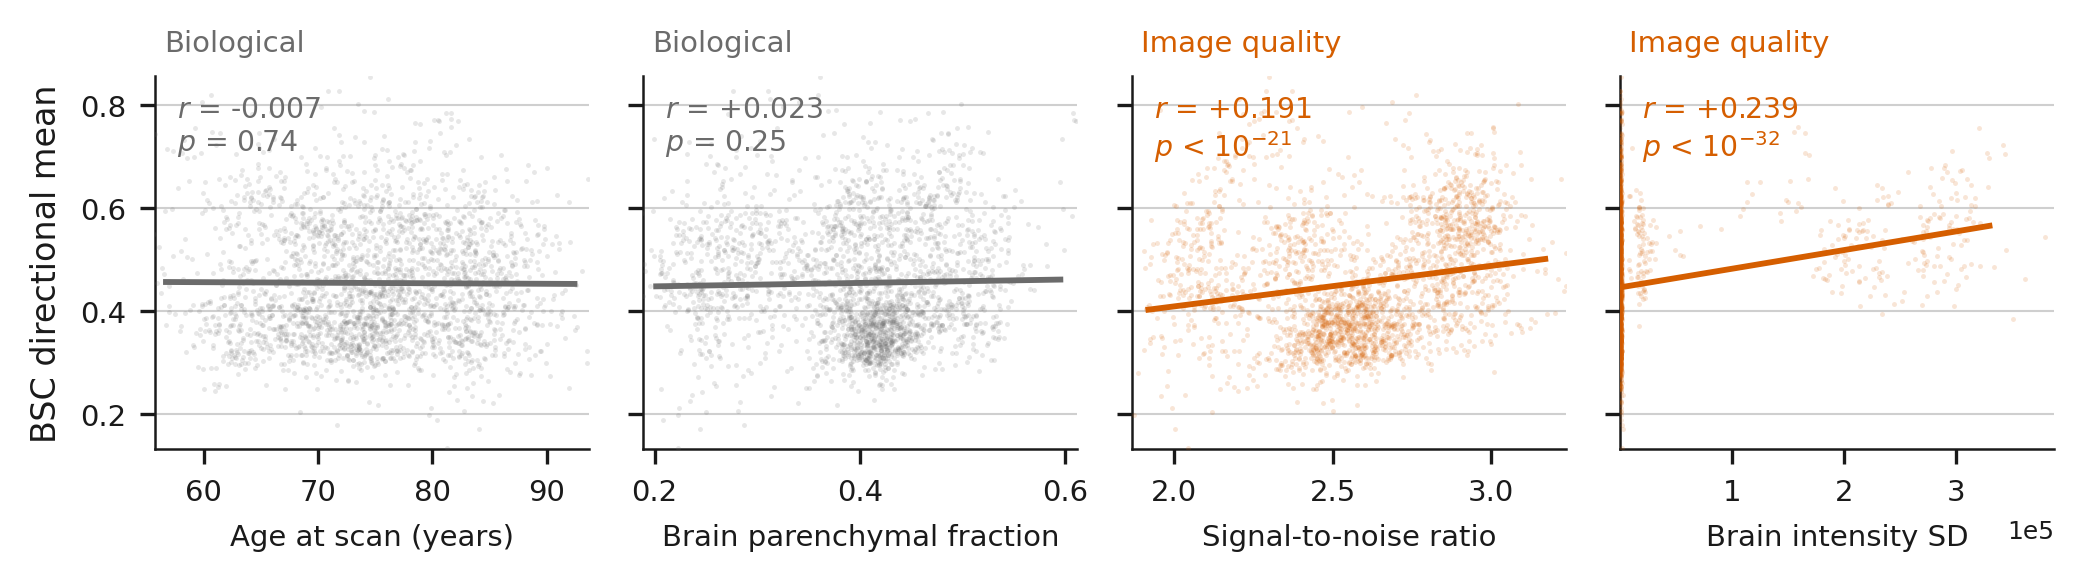
\includegraphics[width=\textwidth]{fig6.png}
\caption{Association between BSC and biological and image quality measures, across the
2,386 cohort scans with complete quality metrics. All four panels use the same scans, so
the contrast is not an artefact of differing sample sizes. BSC shows no association with
age in a cohort of mean age 76.9 years, and none with brain parenchymal fraction, while
correlating with signal-to-noise ratio and with brain intensity dispersion. Gray-white
contrast, the closest established measure, declines detectably with age in healthy adults,
which makes the flat age panel difficult to reconcile with BSC behaving primarily as a
measure of tissue microstructure.}
\label{fig:construct}
\end{figure*}

\subsection{Competing risks}

Death is not rare in a cohort of this age, and the models above treat it as ordinary censoring. Of the 417 subjects, 61 have a death record: 33 died after a dementia diagnosis, which is not a competing event, and 28 died without one. Those 28 are 9.9\% of the 284 subjects counted as censored in the main analysis. Death dates came from an exact withdrawal form for 36 subjects and from a year-only adverse-event field for 25.

Recoding those 28 as competing events changed nothing that matters (Table~\ref{tab:competing}). The cause-specific C-index rose slightly for all three configurations, by 0.016 for clinical covariates, 0.012 for regional BSC slopes and 0.010 for the full set, which leaves the ordering and the gaps between the configurations as they were. On the subdistribution scale the same ordering appears: a standard deviation of the covariate risk score carries a subdistribution hazard ratio of 3.48 (95\% CI 2.70 to 4.87), the full model 2.90 (2.16 to 4.17), and the regional BSC score 1.30 (1.09 to 1.53). Regional BSC is not uninformative on this scale, but it sits far below what the clinical covariates alone deliver, which is the same conclusion the C-index reaches.

Two caveats belong with these numbers. Deaths are recorded a median of 0.95 years after the last clinical visit, so whether a subject converted between that visit and death cannot be observed. And 61 deaths in 417 elderly subjects followed for several years is certainly an undercount, since neither ADNI table captures deaths occurring after a subject leaves the study. The analysis is therefore a lower bound on the competing-event burden. It is enough to answer the question it was run to answer: the null is not an artefact of treating death as censoring.

\begin{table}[htbp]
\centering
\footnotesize
\setlength{\tabcolsep}{4pt}
\caption{Competing-risks sensitivity analysis, gradient-boosted AFT model. Cause-specific C-index follows subjects to the death date and censors there. The subdistribution hazard ratio is per standard deviation of the out-of-fold risk score, with a subject-level bootstrap interval. All 417 subjects enter cross-validation here with no hold-out reserved, so the original column differs slightly from Table~\ref{tab:model-performance}.}
\label{tab:competing}
\begin{tabular}{lccc}
\hline
\textbf{Feature set} & \textbf{Original} & \textbf{Cause-} & \textbf{Fine-Gray} \\
 & \textbf{C-index} & \textbf{specific} & \textbf{sHR (95\% CI)} \\
\hline
Clinical covariates & 0.751 & 0.767 & 3.48 (2.70, 4.87) \\
BSC slopes, regional & 0.615 & 0.628 & 1.30 (1.09, 1.53) \\
Cov.\ + regional + MRI & 0.772 & 0.782 & 2.90 (2.16, 4.17) \\
\hline
\end{tabular}
\end{table}

\subsection{Sensitivity in biomarker-confirmed subjects}

Conversion here is a diagnosis code. Restricting to subjects with confirmed amyloid pathology asks whether the null is a null about Alzheimer's disease or only about a clinical label.

The amyloid-positive subgroup contains 188 subjects with 81 events, and conversion is far commoner in it than outside it: 43\% against 12\% among the amyloid-negative. Inside that subgroup the incremental-value tests give the same answer as the full cohort. Adding global BSC slopes to clinical covariates changed the fold-matched C-index by $+0.024$ (95\% CI $-0.031$ to $+0.092$); adding them to covariates with standard MRI gave $-0.003$ ($-0.051$ to $+0.025$). Regional BSC was worse, at $-0.036$ ($-0.081$ to $+0.057$) over covariates and $-0.073$ ($-0.098$ to $+0.000$) over covariates with standard MRI. The AD-signature composite gave $-0.001$ and $-0.001$. Every interval includes zero, and the regional comparison against covariates with standard MRI only just does, with an upper bound of $+0.0003$.

Everything is measured less precisely here, since 81 events support wider intervals than 133 do, and a small effect confined to biologically confirmed disease would not necessarily show up. What can be said is that restricting to confirmed pathology did not reveal a signal that the diagnosis-code outcome was hiding.

Amyloid status entered as a covariate on the full cohort behaved as expected and changed nothing about BSC. It added 0.005 to the covariate C-index under the flagship model, and with it in the baseline block the BSC increments were $+0.016$ ($-0.009$ to $+0.047$) for global slopes over covariates and $+0.002$ ($-0.013$ to $+0.011$) over covariates with standard MRI, which is where they were without it.

\subsection{Construct validity of BSC}
\label{sec:construct}

Whether BSC adds prognostic value is a question about a model. What BSC measures is a question about the instrument, and it comes first. Five analyses bear on it. Four of them point the same way, and the fifth does not.

\paragraph{Across scans.} What BSC covaries with was checked directly (Figure~\ref{fig:construct}). This check uses every scan belonging to a cohort subject rather than only those inside the feature windows, since the question concerns the measure itself rather than prediction. Of the 2,407 scans contributed by the 417 subjects, 2,386 had complete quality metrics. Across those, BSC showed no association with age ($r = -0.007$, $p = 0.74$ for directional mean). It correlated instead with image quality: brain intensity standard deviation ($r = 0.239$, $p = 3\times10^{-32}$), signal-to-noise ratio ($r = 0.191$, $p = 4\times10^{-21}$) and brain-to-background ratio ($r = 0.133$, $p = 8\times10^{-11}$). Associations with biological measures were weak by comparison, reaching $r = 0.023$ for brain parenchymal fraction ($p = 0.25$) and $r = -0.080$ for brain volume. All six correlations are computed on the same set of scans, so the contrast is not an artefact of differing sample sizes.

\paragraph{Within one brain.} A correlation across scans can be produced by differences between the people scanned rather than by the measure responding to the image. Removing each subject's own mean from both variables answers the stronger question: when the same brain is imaged with more or less noise, does BSC move? It does, and by more than the cross-sectional figure suggests (Figure~\ref{fig:within}, panels A and B). Within subject, BSC rose by 0.297 standard deviations per standard deviation of signal-to-noise ratio (95\% CI $+0.165$ to $+0.429$, $p = 1\times10^{-5}$), against 0.195 between subjects and $r = 0.191$ across scans. Brain intensity dispersion behaved similarly at $+0.116$ within subject ($+0.032$ to $+0.200$). A mixed model with a subject random intercept fitted to the uncentred scans gave $+0.252$ for signal-to-noise ($+0.204$ to $+0.299$), agreeing with the within-subject estimate.

Controlling all time-invariant subject characteristics therefore strengthens the association with image quality rather than weakening it, which is what one would expect if the measure is responding to the image.

The same model shows BSC moving with brain parenchymal fraction within subject, at $-0.324$ standard deviations per standard deviation once age is included. This is a real biological association and it is reported as one. Its sign is difficult to place: boundary sharpness rises as parenchymal fraction falls, so on this reading atrophy would make the gray-white interface crisper. The within-subject age coefficient is likewise positive ($+0.274$), which cannot be read straightforwardly either, since within a subject age is elapsed study time and is therefore entangled with the scanner upgrades ADNI performed over the same years.

\paragraph{Against pathology.} If BSC tracked Alzheimer's pathology, its slopes should correlate with a pathological measure of it. All 159 slopes were correlated against amyloid PET centiloids, CSF A$\beta$42, CSF p-tau, the CSF p-tau to A$\beta$42 ratio and tau PET meta-temporal SUVR. Not one survived false discovery rate control against any of the five targets. The largest correlation with any biomarker anywhere in that screen was $\rho = 0.18$, and the smallest $q$-value against amyloid PET was 0.98. BSC slopes track how the image was acquired and do not track the pathology the outcome is named after.

\paragraph{Scanner signal.} If BSC is partly acquisition signal, acquisition ought to predict the outcome by itself. It does. A Random Survival Forest given nothing but site, vendor and field strength, with 18 indicators in total, reached a cross-validated C-index of 0.609 (SD across folds 0.005), above global BSC slopes at 0.584 and not far below regional BSC slopes at 0.649 (Figure~\ref{fig:within}, panel C). Where and on what a subject was scanned carries real information about whether they converted, which follows from field strength being confounded with the outcome in this cohort and is precisely the structure a longitudinal imaging marker is exposed to.

Residualizing the regional BSC features on that same design matrix, fitted inside training folds, moved the regional C-index from 0.641 to 0.630, a drop of 0.011. The regional signal is therefore not reducible to the coarse acquisition structure that can be modelled here. Two things limit how far that goes. These features have already been through longitudinal ComBat, which removed roughly a quarter of the within-subject step at a scanner change, so much of the scanner variance was gone before the residualizing step. And 18 indicators describe site, vendor and field strength, not the full 120-level batch structure, which cannot be residualized against 417 subjects without removing variance mechanically.

\paragraph{Partial association.} Partialling the image-quality slopes out of BSC's association with conversion did not shrink it. The global BSC slope has a hazard ratio of 0.854 per standard deviation raw (95\% CI 0.691 to 1.055) and 0.842 adjusted (0.679 to 1.046), but neither is distinguishable from unity, so there is nothing there for quality to explain away. The regional risk score does have an outcome association, at 1.516 per standard deviation (1.279 to 1.795), and it did not move when the quality slopes were entered: 1.567 (1.315 to 1.867). Whatever the regional feature set is picking up, the two image-quality slopes available here do not account for it.

\begin{figure*}[t!]
\centering
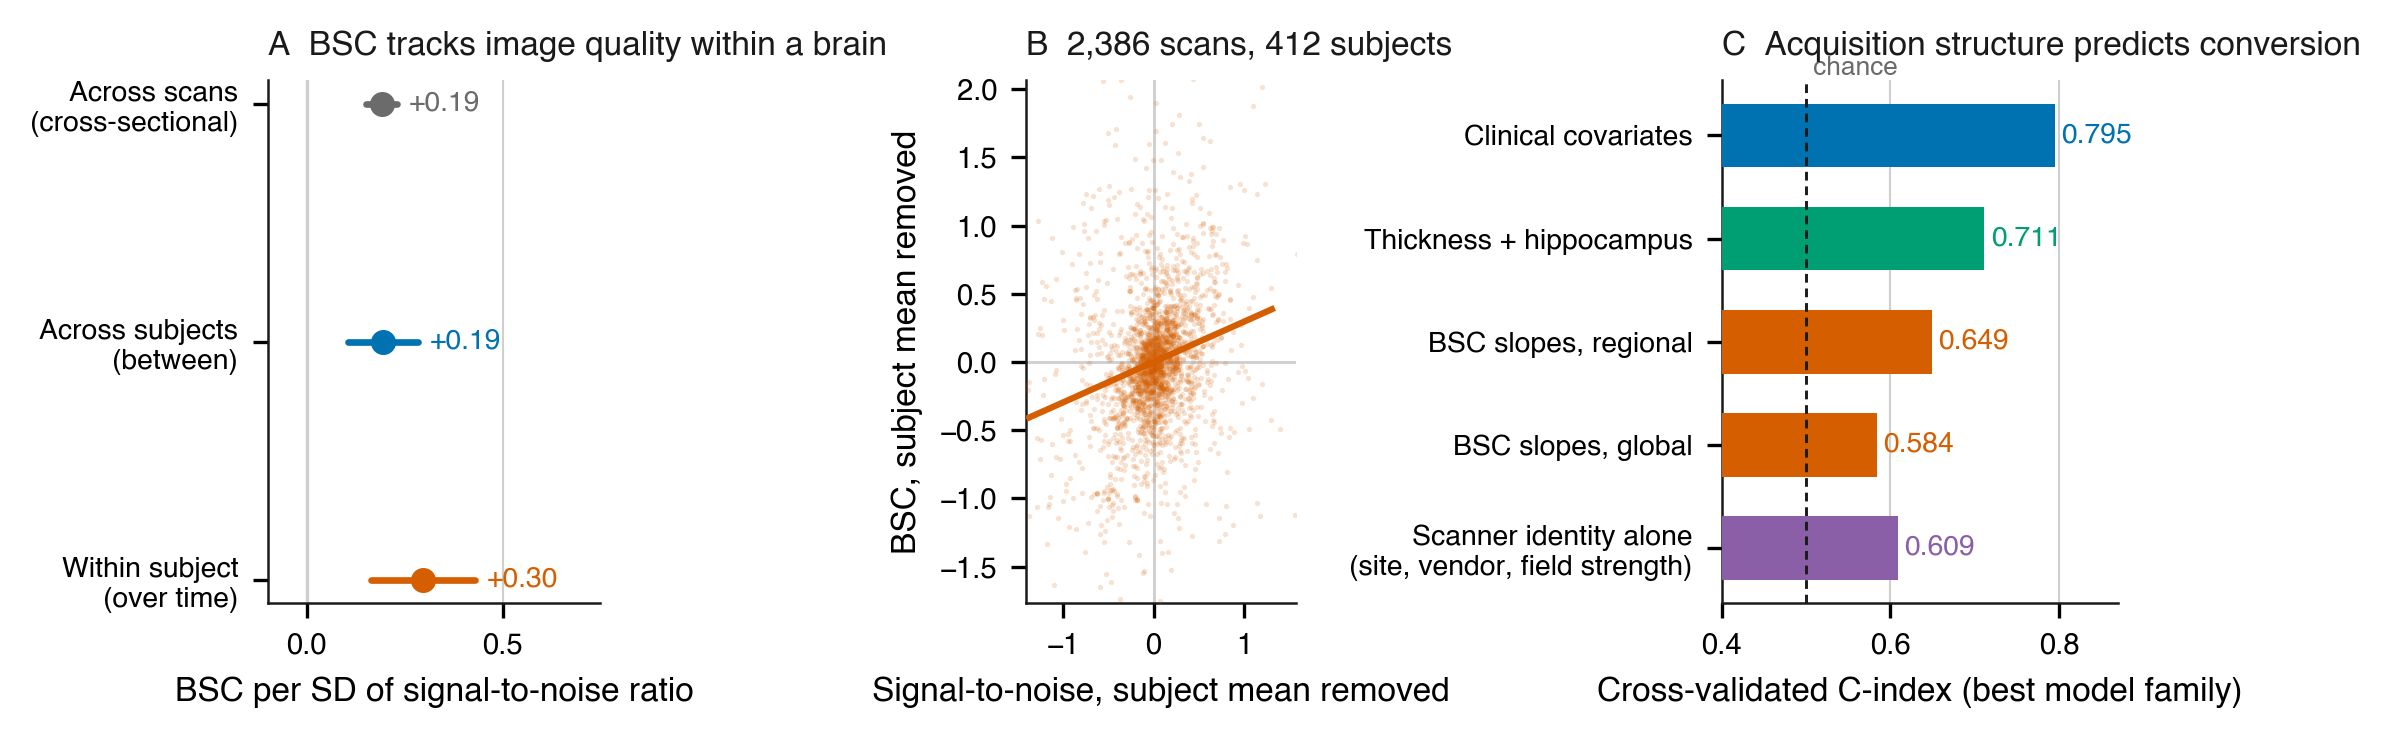
\includegraphics[width=\textwidth]{fig7.png}
\caption{Construct validity of BSC. (A) The association between BSC and
signal-to-noise ratio, estimated three ways, each as a standardized slope with a
95 per cent interval. The within-subject estimate, which removes every
time-invariant subject characteristic, is the largest of the three. (B) The same
within-subject association drawn directly: every scan with its own subject's mean
removed from both axes. (C) Cross-validated C-index for a model given nothing but
acquisition structure, beside the imaging feature sets and the clinical
covariates, each at its best model family. Scanner identity alone discriminates
better than global BSC slopes.}
\label{fig:within}
\end{figure*}

Taken together, BSC does not track age in a cohort old enough that it should, does not track amyloid or tau, tracks image quality more strongly inside one brain than across brains, and is outperformed as a predictor by the scanner label. Gray-white contrast, the closest established measure, declines detectably with age in healthy adults~\cite{salat2009age}. None of this is what a measure of tissue microstructure would look like.

\section{Discussion}

Clinical covariates alone reached a cross-validated C-index of 0.795, above every imaging feature set tested, and every imaging configuration carried a train-to-test gap near 0.20 against roughly 0.02 for the covariate models. Correcting the follow-up definition cost clinical prediction 0.010 to 0.034 in C-index while costing each imaging family two to four times more. No BSC feature set improved on covariates, or on covariates combined with cortical thickness and hippocampal volume. That held when the 28 deaths preceding a dementia diagnosis were treated as a competing event, and it held inside the 188 amyloid-positive subjects. Regional slopes discriminated better than global summaries, 0.649 against 0.584, and of 159 slopes screened, two survived correction for multiple comparisons, both measuring a single region that had not been specified in advance. BSC showed no association with age or with any amyloid or tau biomarker, tracked signal-to-noise ratio more strongly within a single brain than across brains, and was outpredicted by a model given nothing but the scanner label.

That clinical covariates outperform every imaging feature set is unsurprising given what they contain: cognition at the landmark visit, APOE genotype and age. The more informative comparison is the train-to-test gap. Covariate models lost 0.017 to 0.025 between training and held-out folds, whereas every imaging configuration lost close to 0.20, and the fullest combined model trained to 0.984 against a test value of 0.772. With 124 regional features and 106 training events, these models fit fold-specific noise rather than transferable signal, which also explains why the penalized and parametric models on BSC-only feature sets fall below chance out of fold: the risk direction they learn on a training fold does not survive to the fold held out.

The follow-up definition, a form of guarantee-time bias, accounts for most of the apparent prognostic value of BSC slopes. Holding subjects, features and models fixed, correcting the clock left clinical prediction nearly untouched and reduced every imaging family substantially. That asymmetry is the result. A design permitting features from scans acquired after diagnosis inflates longitudinal imaging markers specifically, because those markers can encode disease that has already been diagnosed, whereas cognition measured at the landmark cannot. The effect is not specific to BSC. Cortical thickness and hippocampal volume slopes, which are well validated in AD, were inflated as much, reaching 0.781 with a Random Survival Forest under the original design. Studies proposing longitudinal imaging markers should state explicitly when features were measured relative to the outcome, and this comparison is worth repeating in other cohorts and for other markers, since a design detail that is rarely reported may be shaping published results well beyond this one measure.

Two objections to reading this as a null were tested rather than argued away. The first is censoring. In a cohort of mean age 76.9 followed for years, a subject counted as censored may have died, and 28 of the 284 censored subjects did so before any dementia diagnosis. Recoding them as a competing event moved every C-index up by 0.010 to 0.016 and left the ordering untouched, and the subdistribution hazard ratios reproduce it. The second is biological confirmation. Conversion here is a diagnosis code, and a null against a clinical label is not automatically a null about Alzheimer's disease. In the 188 subjects with confirmed amyloid pathology, where 43\% converted, no BSC feature set improved on covariates either, and the regional set was worse. Neither objection survives, though the amyloid subgroup carries 81 events and cannot exclude a small effect.

Under the corrected design, BSC adds nothing detectable to information already available in clinic. The intervals rule out large effects without excluding a small one, since the widest upper bound reaches $+0.053$, but no BSC feature set produced an increment distinguishable from the one produced by standard volumetric measures over the same folds, and the nested likelihood ratio tests were uniformly non-significant. This is what the prior literature predicts rather than a departure from it. Ansart et al.~\cite{ansart2021predicting}, reviewing 234 experiments, found that cognitive, FDG-PET and electrophysiological measures each improved prediction of MCI progression while T1-weighted MRI did not, and BSC is a T1-derived measure. The practical implication is correspondingly narrow. There is no case for computing BSC slopes in a clinical or trial-enrichment setting at present, and the cost advantage of structural MRI over PET does not bear on a measure that adds nothing once cheaper information is in the model.

Regional slopes outperformed global summaries by 0.065, so collapsing the cortex into a single number discards spatial information and the original global feature set was measurably suboptimal. That advantage did not survive the addition of covariates. Of the 159 slopes screened, the two that survived correction were the left rostral anterior cingulate measured as directional sharpness and as magnitude, which is one region counted twice rather than two independent findings, and that region is not among the seven specified in advance as the AD signature. The pre-specified composite performed at chance. The gray-white boundary marks the transition from cortical neuronal cell bodies to myelinated axonal projections, and synaptic loss, tau pathology, myelin breakdown in superficial white matter and neuroinflammation could each in principle blur it, but a single exploratory hit in a region outside that hypothesis offers no support for any of those mechanisms.

The construct evidence in Section~\ref{sec:construct} is prior to any question about prognostic value. A marker of cortical microstructural integrity in a cohort of mean age 76.9 years would be expected to track age, since gray-white contrast does~\cite{salat2009age}. BSC did not, while tracking signal-to-noise ratio and intensity dispersion more strongly than any tissue measure.

The within-subject analysis is what turns that correlation into an argument. A correlation computed across scans could be produced by the people rather than by the measure: subjects imaged on noisier scanners might differ in ways unrelated to the scanner. Removing each subject's own mean removes all of those differences, and the association with signal-to-noise ratio then gets larger, from $r = 0.191$ across scans to $+0.297$ per standard deviation within subject. When the same brain is imaged with more noise, BSC moves. Pointing the same instrument at pathology finds nothing: none of the 159 slopes correlated with amyloid PET, CSF A$\beta$42, CSF p-tau, their ratio or tau PET after correction. A model given only site, vendor and field strength reached 0.609, above the 0.584 that global BSC slopes reach with 33 features derived from the images themselves.

Two results in this section point the other way and are worth stating plainly rather than filing under limitations. Residualizing the regional features on scanner identity cost only 0.011 in C-index, and partialling the image-quality slopes out of the regional risk score's association with conversion did not shrink it. Neither is strong evidence against the construct argument, since the features had already been harmonized and since 18 acquisition indicators do not capture the full batch structure, but neither supports it. The honest summary is that BSC behaves like a measure of image sharpness in every direct test of what it tracks, while the residual discrimination of the regional feature set is not fully explained by the acquisition variables available here.

This separates BSC from the boundary measures it resembles. Gray-white contrast is a ratio of sampled intensities and is comparatively robust to overall gain, whereas a spatial derivative of intensity responds to sharpness of the image as well as sharpness of the anatomy. Blurring measures in the epilepsy literature control for this by z-scoring against a normative database acquired on matched hardware~\cite{huppertz2005enhanced,blackmon2015cortical}, which a longitudinal multi-site design makes difficult. Whether a formulation that normalizes for local image sharpness retains biological signal is the most direct next step. If a normalized variant recovers the age association, the measure is worth revisiting; if it does not, that is informative in its own right.

Several limitations qualify these results. The first is that every analysis here is within ADNI. A single cohort can show that a design choice changes an answer, and it can show that a marker fails to add value in the cohort where it was proposed, but it cannot establish that either finding generalizes. Replication in an independent cohort is the most important next step, and the design-effect comparison is the part most worth repeating, since it applies to any longitudinal imaging marker and not to BSC alone. That work is not attempted here and nothing above should be read as external validation.

Death ascertainment rests on ADNI registry and adverse-event records, and those are incomplete. Only 61 of 417 subjects carry any death record, which in a cohort of this age and follow-up is certainly an undercount, since neither table captures deaths after a subject leaves the study. Twenty-five of the 61 death dates are de-identified to a year and were placed at its midpoint. Deaths are recorded a median of 0.95 years after the last clinical visit, so conversion between that visit and death is unobservable. The competing-risks analysis is a lower bound on the competing-event burden rather than a full accounting of it.

Amyloid coverage differs between the outcome groups, at 76\% of converters against 89\% of stable subjects. The untested subjects are largely ADNI1 participants enrolled before amyloid PET entered the protocol, and ADNI1 also had the highest conversion rate, so status is missing for a reason connected to the outcome. The amyloid-restricted analysis is a sensitivity analysis for that reason, and its 81 events support wider intervals than the main analysis does.

Motion was not assessed, since the pipeline computes signal-to-noise and related intensity statistics but no motion estimate. Given the sensitivity of BSC to image quality reported here, motion is a plausible contributor that this study cannot quantify: BSC is characterized against three intensity-based quality metrics and against none that measure how still the subject was. Scanner harmonization is incomplete: longitudinal ComBat removed roughly a quarter of the within-subject step at a scanner change, and because field strength is confounded with conversion status in this cohort, the residual variance is correlated with the outcome rather than being random noise. Parcellation quality depends on vendor, with boundary-band coverage falling below 5\% for 32.6\% of scans from one manufacturer against 9.2\% and 0\% for the other two, so regional feature quality is not missing at random; all scans were retained and coverage carried as a quality metric rather than used to exclude, because exclusion would import that bias directly.

Sample size limits several analyses. The hold-out contains 27 events, too few for a precise estimate, and the largest feature sets contain more features than there are events, so the cross-validated performance estimates are trustworthy while per-feature interpretation of those models is not. BSC is defined relative to Atropos probability maps, so segmentation instability propagates into the measure.

In 417 ADNI subjects with 133 conversion events, longitudinal BSC slopes added no prognostic information beyond clinical covariates and established longitudinal MRI measures once follow-up was defined so that every feature preceded the outcome. Adding regional BSC slopes to covariates and standard MRI changed the fold-matched C-index by 0.002 (95\% CI $-0.021$ to $0.022$). That result survived treating death as a competing event and restricting to biologically confirmed disease. Comparing the two designs on the same subjects, the corrected definition cost clinical prediction almost nothing and cost every imaging feature family several times more, including measures that are well established. The prognostic value previously reported for BSC slopes is therefore better attributed to the analysis design than to the biomarker. The construct evidence points the same way: BSC tracks signal-to-noise ratio more strongly inside a single brain than across brains, tracks neither age nor amyloid nor tau, and predicts conversion less well than the scanner label does. Both questions about the construct come before any question about its clinical use.

\begin{acknowledgments}
Data collection and sharing for the Alzheimer's Disease Neuroimaging Initiative (ADNI) is funded by the National Institute on Aging (National Institutes of Health Grant U19AG024904). The grantee organization is the Northern California Institute for Research and Education. In the past, ADNI has also received funding from the National Institute of Biomedical Imaging and Bioengineering, the Canadian Institutes of Health Research, and private sector contributions through the Foundation for the National Institutes of Health (FNIH) including generous contributions from the following: AbbVie, Alzheimer's Association; Alzheimer's Drug Discovery Foundation; Araclon Biotech; BioClinica, Inc.; Biogen; Bristol-Myers Squibb Company; CereSpir, Inc.; Cogstate; Eisai Inc.; Elan Pharmaceuticals, Inc.; Eli Lilly and Company; EuroImmun; F. Hoffmann-La Roche Ltd and its affiliated company Genentech, Inc.; Fujirebio; GE Healthcare; IXICO Ltd.; Janssen Alzheimer Immunotherapy Research \& Development, LLC.; Johnson \& Johnson Pharmaceutical Research \& Development LLC.; Lumosity; Lundbeck; Merck \& Co., Inc.; Meso Scale Diagnostics, LLC.; NeuroRx Research; Neurotrack Technologies; Novartis Pharmaceuticals Corporation; Pfizer Inc.; Piramal Imaging; Servier; Takeda Pharmaceutical Company; and Transition Therapeutics.

Computations were performed on the Trillium cluster at SciNet, University of Toronto. The author thanks Dr. Fabrizio Piras (IRCCS Santa Lucia Foundation, Rome) for valuable discussions on longitudinal modeling strategies, and the open-source neuroimaging community for developing ANTsPy, nibabel, scikit-survival, lifelines and related tools that made this work possible.
\end{acknowledgments}

\section*{Data availability}

The imaging and clinical data analysed here are available from the Alzheimer's Disease Neuroimaging Initiative (\texttt{adni.loni.usc.edu}) to investigators who register and are approved under the ADNI Data Use Agreement. The author received no special access privileges. All analysis code, covering cohort construction, harmonization, modelling, the competing-risks, biomarker and construct-validity analyses reported here, and figure generation, is publicly available at \texttt{github.com/ishaan-cherukuri/research/tree/main/mri-bsc}. Every analysis uses random seed 42 and the frozen 417-subject cohort, and the sensitivity analyses reuse the cross-validation folds of the primary models rather than resplitting.


%% References using BibTeX
\bibliographystyle{unsrt}
\bibliography{references}

\end{document}
